\documentclass[class=NCU_thesis, crop=false, float=true]{standalone}

\begin{document}
\let\orilabel\label % enable \ref in LTXexample

\chapter{FAQ}
\label{sec:c_faq}
\section{什麼是\LaTeX ?}
\LaTeX\  是一個非常古老、強大、專業的排版軟體。它將許多專業排版的細節隱藏起來
\footnote{專業排版連\SI{0.2}{\milli\metre}都在苛求。}
,讓你專注在內容上而不用擔心最終文件是否好看。這一個特性又以數學公式最為顯著(用Word的應該可以深切體會微軟對於防止客戶腦袋老化的用心良苦 :D )。

使用上來說,\LaTeX\ 使用過程如同寫程式般,須要用一些指令告訴\LaTeX\ 這段文字是什麼(標題、章節......)。最後還要經過編譯才能看到排版結果
\footnote{雖然部份編輯器提供即時編譯功能,只要停止輸入幾秒立刻進行編譯。但實務上這不是必要的,並且會加重電腦的負擔。另外有些如Lyx這類「所見即所得」(WYSIWYG)的軟體是基於\LaTeX\ ,各位可以玩玩看。}
。這種非「所見即所得」(WYSIWYG)的軟體可能會讓許多新手敬而遠之。不過不用擔心,你已經拿到這份教學了,一定可以在1hr內學會寫\LaTeX\ 文件的 :D !

\section{\LaTeX 比起 Word 有什麼優點?}
\begin{itemize}
    \item 文字間距以及字本身大小不是固定的,它會做微幅調整讓整體最為美觀。這點在英文上更為明顯(Microtype套件能做到更漂亮)。
    \item 圖表位置可以浮動,能夠限制圖表只能在頁頂或頁底,不用再擔心插入文字會跑掉。
    \item 程式化特性,讓許多重複文字、動作都可以簡化。
    \item 數學公式美觀,輸入更為方便、穩定,不會像Word無法理解的跑來跑去。
    \item 站在巨人的肩膀上。\LaTeX\ 為出版界所用,排版規則即為專業規範。
    \item 隨時隨地寫論文,因為只要簡單的文字編輯器即可,任何智慧型手機、平板均可寫作。
    \item 免費正版,不會好心的告訴你「你是盜版的受害者」。讓你專心寫論文。
\end{itemize}

\section{新手如何學\LaTeX\ ?}
\begin{enumerate}
    \item 砍掉Windows... 喔不,是忘了 Word。\LaTeX\ 不是Word,也不是單純的記事本。請不要用Word 的方式去使用\LaTeX\ 。(其實很多人把Word當記事本用....)
    \item 快速瀏覽過本教學。不懂沒關係,至少知道\LaTeX\ 有哪些功能、要到哪裡找。瀏覽一遍只要15分鐘,不知道好用功能可以浪費你好幾天。(\emph{學弟妹們!不要再手打圖表編號了啊!!})本教學不會是最好的\LaTeX\ 教學,不過我相信對中文使用者來說,這是非常好入門的教學。至少足夠你寫論文了!
    \item 實踐中學習。快寫論文吧!
\end{enumerate}

\section{這樣板和中央大學(羅吉昌先生)提供的有何不同?}
嗯.... 這對我來說是能否編譯的差別 XD 。 原因我也不知道為何,不過不少同學即使能夠產生PDF檔,也還是須要修改一些小地方。所以我乾脆就把我從頭打造的設定做成樣板啦!
\footnote{其中還是有很小一部份是修改自羅吉昌的樣板,譬如封面頁的格式幾乎就是羅吉昌的。}
我寫論文時選定的編譯器是\XeLaTeX\  ,理由是他可以直接使用系統內的字型,也對非拉丁文字支援較好的樣子。所以這個樣板完全只測試\XeLaTeX\ 下的使用情況。

除了專注在\XeLaTeX\ 之外,我的版本也儘量使用套件處理格式而不直接動底層的設定。
\footnote{2016/10/26: 為了符合學校要求,還是重定義了一些\LaTeX\ 指令......}
譬如版面設定直接使用geometry 套件設定邊距。這麼做除了我本身不熟\LaTeX\ 外,也相當於將底層的轉換交給套件開發人員,會比我自己維護來的好得多。我也替換掉將數字轉成中文(1 $\rightarrow$ 一、2 $\rightarrow$ 二)的xCJKnumb而改用zhnumber。這是因為xCJKnumb為CJKnumb的改造版,而這個套件不存在於ctan網站上,要取得只能google,然後在不知名blog上下載。雖然目前使用上沒有問題,但未來維護則未知。

\section{這樣板符合學校要求嗎?}
先說結論,我的論文是照此格式提交的,既然審過了,應該沒有問題。
\footnote{其實中央很松啦~~我看過比我更慘的格式。\textbf{重點在內容啊!}}

這樣板並非完全照學校要求製作。理由是有些規定我認為過於於愚蠢或是使編排變得混亂。差異處如下:
\begin{itemize}
    \item 附錄編號採用英文字母A,B,C。理由:附錄編號與正文不該相同。(羅先生樣板雖然表面符合學校格式,但實在不應該讓章條目是中文,節條目出現英文A.1。)
    \item 節編號的連接符「-」換成「.」。理由:1. \LaTeX\ 預設。 2. 表達較為清晰、美觀。 3. 沒看過用「-」的。
    \item 圖、表、公式全部以章分別編號。理由:1. \LaTeX\ 預設。 2. 這樣做更能了解內容類別。
    \item 參考文獻格式使用 Nature 風格。理由:國際通用、製作方便。
\end{itemize}
另外還有章節風格的問題,請見\cref{sec:s_specialTemplate_ncu_secStyle}。

\section{這樣板有很厲害嗎?}
我最初大概花了1個月左右來調樣板吧!(然後教學又是1個多月......)有很多小細節都已經解決了,也儘量做到自動化設定(連pdf屬性都貼心的幫你完成了呢!\cref{fig:pdf_metadata.png})。當然啦!花費時間跟天資也是有關的,你要說「這東西也要花一個月?」我也認了orz......
\fig[0.7][][t]{pdf_metadata.png}
\footnote{持續更新中==持續花時間......}

\section{要怎麼使用樣板?}
{\color{red}
    樣板詳細設定方法使用GitHub 專案的wiki頁面做說明。
}

整個流程如下:
\begin{enumerate}
    \item 照教學檔安裝、設定軟體環境。修改編輯器的預設LaTeX編譯器,\textbf{改成使用\XeLaTeX\ }。與文獻資料庫處理程式\textbf{(改成使用biber)}。
    \item 先編譯一次樣板或是教學檔中的\textbf{根文件(main.tex)},確認正常編譯。\textbf{編譯前先修改config.tex中的中文字型或作業系統,詳情見\cref{sec:s_template_structure}。}\footnote{這部份其實可以透過ifplatform套件自動解決,但須要加入``-shell-escape''參數至編譯指令,我怕新手對這比較怕,所以改用設定值處理。}如果編譯出錯的話建議自行找人解決,沒人解決可以找我。不過畢竟不在現場,處理上會較為麻煩。自行解決後請回報問題及解法。
    \item 依樣畫葫蘆。
    \begin{enumerate}
        \item 設定(各學校目錄中的)config.tex中的個人資訊以及相關設定。
        \item 照教學檔試著插入文字、圖檔、表格......至以存在的chapter\_開頭的檔案。(圖片檔、程式碼檔案請置入figures、codes目錄中。)
        \item 須要新增章節子檔的話直接複製chapter\_template(\_demo).tex,修改內容、重命名後插入main.tex對應的章節位置。
        \item 要新增使用套件或其他導言區指令請填入 macros\_preamble.tex檔案,樣板會自動讀取。文獻資料庫bib檔一樣於此檔中設定。
        \item 同樣的,文件內的共用指令(填在\textbackslash{}begin\{document\}之後的)填入macros\_document.tex。
        \item 若有風格不符合的部份(如:文獻引用要用作者名、列表要照字母排序等等),請於cls檔中搜尋關鍵字(編輯器通常會提供搜尋功能,或按快速鍵Ctrl+f),找到設定行之後自行修改。
    \end{enumerate}
    \item 全部完成後編譯main.tex,產生pdf。
    \item 口試後將審定書、推薦書等文書簽名後掃描後存成pdf置換原先插入的單頁pdf。(附件區域已嘗試自動生成客製化文件,省去另開Word編輯文件的功夫。)
\end{enumerate}
論文各文件、章節次序已經按照學校要求排好,各位只要直接修改或替換即可。

\section{樣板不符合我的要求怎辦?}
要新增使用套件或其他導言區指令請填入 macros\_preamble.tex檔案,樣板會自動讀取。文件內的共用指令(填在\textbackslash{}begin\{document\}之後的)填入macros\_document.tex。一些設定要改的話可於cls檔中搜尋關鍵字(編輯器通常會提供搜尋功能,或按快速鍵Ctrl+f),找到設定行之後自行修改。

如果遇到(其他)學校要求一些奇奇怪怪的格式,真的不會改的話,只好用其他軟體(LiberOffice Writer,甚至是LiberOffice Draw)先生成pdf檔再插入囉!
        
\section{有其他教學嗎?}
\LaTeX\ 教學很多,但大多是英文的。免費資源中,wikibook的\LaTeX\ 
\footnote{\url{https://en.wikibooks.org/wiki/LaTeX}}
是我非常推薦的,同時也是本文主要參考的文件。
中文的完整文件有\LaTeX\ 123
\footnote{\url{http://www.cs.pu.edu.tw/~wckuo/doc/latex123/node1.html}}。
不過文中使用的是\LaTeX\ + CJK套件,而本文用的是\XeLaTeX\ ,少數內容與本樣板不同。
另外還有cwTeX的文件也可以參考。

如果你碰到問題,研究半天無解,想問人沒人問又不想上英文論壇問,可以上ptt的 LaTeX 板試試。(那裡臥虎藏龍啊!)

\section{MATLAB 圖要如何插入?}
不管你是用MATLAB還是Origin還是其他軟體生成的圖,都要匯出成一般圖檔才能插入。建議格式依序為為eps、png、jpg。
\footnote{eps是向量圖,縮放不失真,同時也是\LaTeX\ 原本就支援的格式。png, jpg則是\XeLaTeX\ 才支援。}
如果是流程圖或一些手繪線條圖,雖然\LaTeX\ 有套件可以畫出,但我建議初學者還是用Dia/LibreOffice Draw之類的,先畫完再匯出成eps插入比較快。

\section{編譯出錯怎辦?}
看錯誤訊息囉!首先回憶你剛剛做了什麼。接著儘量減少錯誤的可能,把新增行一一註解掉。有必要的話新增一個空的子檔,把新增內容複製過去檢查(會比編譯整份文件快得多)。
如果自己找不出解決辦法,試著把錯誤訊息拿去google看看。

\section{為什麼你的樣板沒有附書脊(側邊)?}
目前還沒做,實際上也不須要。校園四周影印店的人比你我還專業!(我不清楚書皮製作流程,影印店也有可能為了方便製作根本不用你的書脊。)

\section{台大有規定要加密、保全,為什麼你沒有?}
{\color{red}因為我認為加密完全沒有用,最後害到的只有你的讀者。}如果你的論文真有極高價值,就是花錢請人重打一份都可以。或是直接OCR也可以獲取文章資訊,所以最好的保全方式就是根本不要拿出來。最終,你的加密只會讓不去破解的使用者感到麻煩而已。看看影音公司為了防止盜版做了多少加密措施,結果要盜的人直接轉錄去除加密。而乖乖牌使用者則要忍受一堆限制,還有未來可能無法使用的問題。
\footnote{DRM, \url{https://zh.wikipedia.org/wiki/\%E6\%95\%B0\%E5\%AD\%97\%E7\%89\%88\%E6\%9D\%83\%E7\%AE\%A1\%E7\%90\%86}}
同樣的,Windows使用者因為沒連網就要被抹黑使用盜版,而破解版爽爽用~~(還好我用Linux,沒這問題:D)

\section{為什麼你的\LaTeX 歪歪的啊!}
這是\LaTeX 的logo,本來就是\textit{歪歪}的。你可以用\textbackslash{}LaTeX 指令做出。注意大小寫以及後面要有空格區別指令與後方文字。英文環境下要再後面加一個反斜線像這樣:\verb*|\LaTeX\ |,不然因為空格被當分隔字元,\LaTeX\ 會和後面文字黏在一起。

\section{為什麼你一直Linux Linux的啊!}
正啊! lol \\
只有和她好好相處一個月才會發現她的好,也才會發現她是無可取代的。 \\

\noindent 要試嗎? :D



\chapter{軟體安裝}
\label{sec:c_install}
目前主要針對Linux、Windows下的軟體做說明。(Mac也有相對應軟體,但僅稍微提及)
\section{TeX 編輯器}
雖然TeX 檔均為純文字檔,用任何一個文字編輯器均能編輯(即使是windows的記事本)。但選用一個好的Tex 編輯器可以省下不少功夫,像是快速鍵編譯、語法高亮度、原始碼片段插入,也會比爛爛的Windows記事本還安全,像是自動儲存等等。以下列表前兩者為我推薦的編輯器:
\begin{enumerate}
    \item TexStudio , 跨平台的編輯器,具有許多好用功能,並且仍在活躍開發中,非常推薦\footnote{Linux/Windows/Mac均有。也是眾多Macer的選擇}。(此為Texmaker 的分支版)
    \item Kile , KDE下的編輯器,我用的是這個。
    \item Gummi , 一個可以即時編譯的編輯器。
    \item TeXShop, Mac上的另一個選擇。(沒用過,自己試) 
\end{enumerate}
關於編譯時的行為,TexStudio與Kile兩者都能夠自動找到根文件(將整份文件分割成不同tex檔撰寫時,最上層的主文件)進行編譯。TexStudio毋須任何設定,Kile則須要將檔案加入專案中。此功能好處是編輯任何子文件後,直接按下編譯快速鍵即可完整編譯整份文件,不過缺點是浪費時間。如果你有用到subfile/standalone等輔助套件可以考慮禁用此功能,也不須修改根文件的內容。(我在Kile 的作法是除了main.tex外,全部加入專案做管理,按編譯後由於kile找不到引用的上層文件,所以就會只編譯當前檔案。)

TexStudio 由於持續開發的緣故,支援了很多有趣的東西。像是``magic comments'',可以在Tex檔開頭利用註解指定一些編譯參數,當使用支援的環境編譯時,就不須手動選擇使用\XeLaTeX\ 或是手動插入編譯所須參數。

\section{TeX 發行版}
所謂「發行版」指的是特定組織將編譯TeX所須的環境,包含編譯器、常用套件等等包裝在一起發佈的軟體集合。最流行的三個分別是TeX Live、MiKTeX、MacTeX 。 TeX Live 設計上是朝多人使用設計(應該是指安裝在伺服器上共用),而MiKTeX 則是單人使用,所以在安全性方面TeX Live 會較好,詳情請自行google。以下是其官方網站:
\begin{itemize}
    \item TeX Live \url{https://www.tug.org/texlive/} Linux/Unix, Windows
    \item MiKTeX \url{http://miktex.org/} Windows
    \item MacTeX \url{http://www.tug.org/mactex/} Mac
\end{itemize}
\LaTeX\  網站上對此亦有詳細列表,甚至包含了幾個線上版的TeX(\url{https://www.latex-project.org/get/})。下面介紹不同作業系統下的安裝方法。

\subsection{GNU/Linux}
一般來說Linux儘量由(Linux)發行版自己的套件庫安裝會比較好,這裡以 Debian 的指令模式舉例,視窗介面或是其他發行版請自行舉一反三。

以下是我在Debian 中須要手動安裝的套件,其他須要安裝的會透過相依性自己安裝。(如果想全裝就裝texlive-full套件)
\begin{table}[h]
    \centering
    \begin{tabular}{|l|l|}
        \hline
        套件名稱(in debian)     & 說明及需求TeX套件 \\ \hline
        texlive                & 主要套件,會連帶安裝基本系統 \\ \hline
        texlive-bibtex-extra   & BibLaTeX      \\ \hline
        texlive-lang-chinese   & xeCJK,連帶安裝CJK相關套件  \\ \hline
        texlive-science        & siunitx(單位)   \\ \hline
        texlive-xetex          & \XeLaTeX\          \\ \hline
        biber                  & 搭配BibLaTeX   \\ \hline
    \end{tabular}                                      
\end{table}

對應的一行安裝指令為
\begin{lstlisting}[style=consoleStyle,language=bash]
apt-get install texlive texlive-bibtex-extra texlive-lang-chinese
\end{lstlisting}

稍微注意一下 lmodern 套件是否自動安裝,我在debian 7上面碰過沒自動裝,導致找不到字型的問題。(這套件包含一些英文PS字型(Latin Modern family),自樣板1.6版後預設使用它)

稍微說明一下,我的樣板使用\XeLaTeX\  + Biblatex + biber 。如果要用傳統的Bibtex 做文獻索引的話免裝texlive-bibtex-extra biber。

缺套件時除了google後安裝含所須tex套件的Linux套件這個方法外,也可以使用Tex Live自己的套件管理程式tlmgr來安裝單一套件。

\subsection{Windows}
請上各\LaTeX\ 發行版官方網站下載。安裝內容若不知如何選請按完整安裝或是日後透過Tex Live自己的套件管理程式tlmgr進行安裝(目前的TeX Live全裝約4.5GB。)。MiKTeX 具有即時安裝的功能,編譯時若有缺會自動下載。

\section{文獻資料庫(.bib)管理軟體}
如果你的文獻列表使用到文獻資料庫(.bib)的話,建議你安裝一個管理軟體比較方便。這節的說明若看不懂可以先跳到基礎教學的文獻(\cref{sec:s_bib})看一下。
先列出常用的文獻管理軟體:
\begin{description}
    \item[Zotero] 極度推薦!同時也是我使用的文獻管理軟體。免費、自由(AGPL授權)、開源、跨平台、Unicode(可引入中文條目)。加上BBT擴充後可以方便的插入\textbackslash{}cite\{cite\_key\}。(下面專門介紹)
    \item[JabRef] 使用Java開發,免費、自由(MIT授權)、開源、跨平台、似乎支援Unicode,但須手動設定。可以方便的插入\textbackslash{}cite\{cite\_key\}。
    \item[Bibus] 很早期的Linux軟體介紹會出現,但個人感覺頗難用,且已停止開發。
    \item[KBibTeX] KDE (Linux的桌面環境之一)提供的漂亮軟體。沒用過XD,用KDE有興趣玩玩。
    \item[EndNote] \$ \$ \$ 。非常昂貴的軟體(我知道各位的學校、研究單位都已經很好心的幫我們繳錢了,這點可能不是問題...)。不支援中文、不支援Linux。個人不推。
\end{description}
我自己用的是Zotero,所以在這裡詳述心得。
Zotero 有Firefox addon 版以及Standalone版
\footnote{亦有Chrome 和Safari版,見\url{https://www.zotero.org/download/}}
。我是兩個都裝,因為Firefox addon 版可以在瀏覽網頁的當下點addon 提供的按鈕,直接匯入網頁、期刊的文獻資料,省去慢慢手打的時間。這方面其他文獻管理軟體就沒這麼方便。
\footnote{期刊可以使用google scholar各條目下的「引用」複製所須資訊(如BibTeX、EndNote)再匯入管理軟體,。 EndNote 本身則是提供搜索引擎,可以直接取得相關資訊。}
。
而Standalone版的好處則是操作快速,當然這可能跟我的Firefox有1000+個分頁有關,各位可自行決定是否加安裝Standalone版。

\LaTeX\  引用文獻時須要使用\textbackslash{}cite\{cite\_key\}這樣的指令,但對於大量文獻,我們很難記得每一個的cite\_key(有些編輯器支援自動補完,但仍須記得前幾個字母),所以文獻管理軟體要是能支援插入\textbackslash{}cite\{cite\_key\}是一件非常美好的事,這也是我朋友極力推薦 JabRef 的原因之一。 Zotero 雖然本身不提供這個功能,但透過\textbf{B}etter \textbf{B}ib(La)\textbf{T}eX 擴充後能夠以拖曳方式插入\textbackslash{}cite\{cite\_key\} 。

\subsection{安裝Zotero以及BBT套件}
Zotero 可由官網\url{https://www.zotero.org/}下載。而BBT擴充的專案位於\url{https://github.com/retorquere/zotero-better-bibtex}。安裝說明頁 \url{https://github.com/retorquere/zotero-better-bibtex/wiki/Installation} 其中的xpi檔連結即為BBT套件,下載並安裝至Zotero/Firefox。

安裝完畢後開啟Zotero 設定視窗,在「匯出」分頁的「預設輸出格式」選「Better BibTeX Quick Copy」即可使用拖曳插入\textbackslash{}cite\{cite\_key\} 的功能。
\fig[0.7][][h]{tutorial_zotero_bbt_config.png}[BBT拖曳插入cite\_key的設定方法。]
\subsection{Zotero使用方法}
Zotero 的一個最方便的地方就是直接由瀏覽器匯入所須資訊。\cref{fig:zotero_save}為儲存一篇\emph{Nature}期刊的例子。只要在Firefox上點一點,不但儲存作者、期刊標題等資訊,連pdf檔都一起存進來了呢!(當然你要有權限才可以啦!還有像APS系列期刊還要先朝\emph{愛因斯坦}三鞠躬才準載喔!)
\begin{figure}
    %\captionsetup[subfigure]{labelformat=empty} % 完全隱藏圖號
    \centering
    \subcaptionbox
        {點紅框處儲存
        \label{fig:Zotero_01}}
        {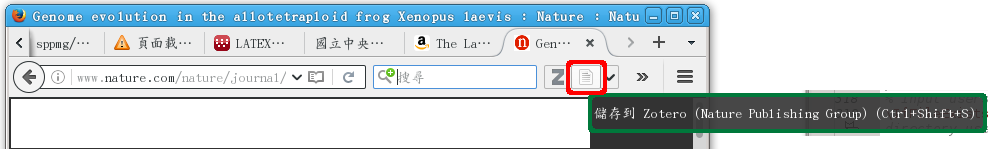
\includegraphics[width=0.95\linewidth]{Zotero_01.png}}
        
    \vspace{\baselineskip}
    \subcaptionbox
        {儲存中(螢幕右下角)
        \label{fig:Zotero_02}}
        {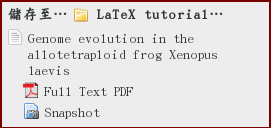
\includegraphics[width=0.4\linewidth]{Zotero_02.png}}
        
    \vspace{\baselineskip} % 分隔上下列
    \subcaptionbox
        {完成
        \label{fig:Zotero_03}}
        {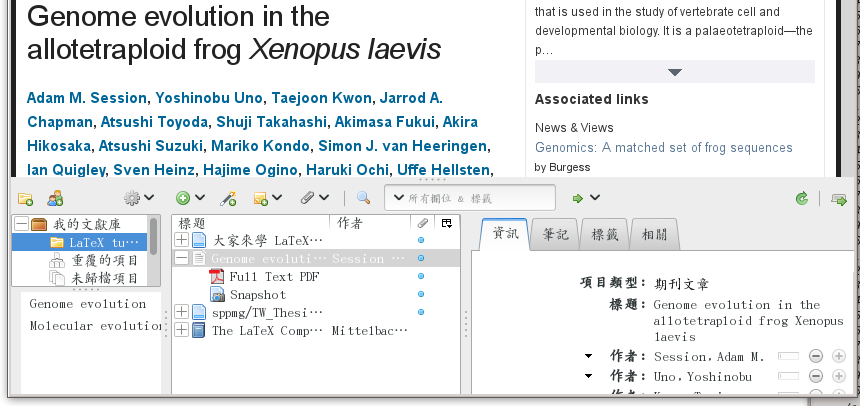
\includegraphics[width=0.95\linewidth]{Zotero_03.png}}
    
    \vspace{\baselineskip} % 分隔上下列
    \subcaptionbox
        {資料庫項目
        \label{fig:Zotero_04}}
        {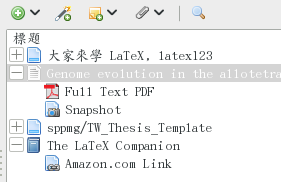
\includegraphics[width=0.4\linewidth]{Zotero_04.png}}
    \hspace{0.8cm}
    \subcaptionbox
        {條目資訊
        \label{fig:Zotero_05}}
        {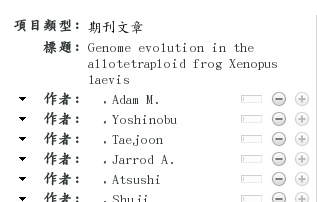
\includegraphics[width=0.4\linewidth]{Zotero_05.png}}
    \caption{Zotero 儲存期刊資訊}
    \label{fig:zotero_save}
\end{figure}

最後要編譯前記得對Zotero中的文獻庫(左方窗格的資料夾圖示)按滑鼠右鍵,選「匯出文獻庫」並選擇「BibLaTeX」格式(如果你打算採用BibTeX格式請記得自行修改樣板)匯出.bib文獻庫。如\cref{fig:zotero_exportBib}
\footnote{JabRef這類直接對.bib進行管理的軟體應該就不須要再匯出了。}
\begin{figure}
    %\captionsetup[subfigure]{labelformat=empty} % 完全隱藏圖號
    \centering
    \subcaptionbox
        {匯出文獻庫(選定的目錄)
        \label{fig:Zotero_06}}
        {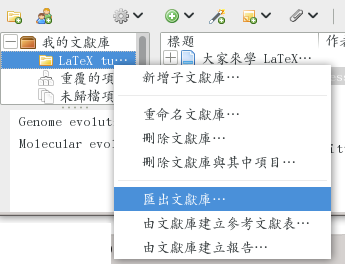
\includegraphics[width=0.4\linewidth]{Zotero_06.png}}
    \hspace{2em}
    \subcaptionbox
        {匯出BibLaTeX格式(本樣板採用BibLaTeX)
        \label{fig:Zotero_07}}
        {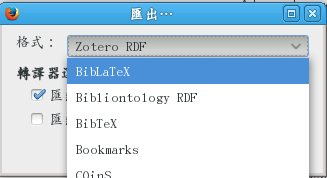
\includegraphics[width=0.4\linewidth]{Zotero_07.png}}
    \caption{Zotero 匯出文獻資料庫bib檔}
    \label{fig:zotero_exportBib}
\end{figure}

\section{本\LaTeX\ 專案結構及使用說明}
這節的說明若涉及到\LaTeX\ 專有名詞請先閱讀後面教學。
\subsection{取得專案}
本專案公開於GitHub,你可以在``TW\_Thesis\_Template''專案首頁\cite{_sppmg/tw_thesis_template_????}(不是我的帳號首頁喔!)右邊找到Download鈕(\cref{fig:github_pjDownload.png})下載整個專案(github不提供下載單一目錄。單檔可以進入頁面後另存)。下載前確認你要載的版本,左側``Branch''鈕可以選擇不同的分支(\cref{fig:github_branchList}),master分支通常是穩定版,而有時為了測試會新增develop分支。``tag''則是在重要版本發布時(Ver 1.0)才會特別標記(\cref{fig:github_tagList})。
\fig[0.5]{github_pjDownload.png}
\begin{figure}
    \centering
    \subcaptionbox
        {GitHub 分支列表(使用我的另一個有develop分支的專案當範例)。
        \label{fig:github_branchList}}
        {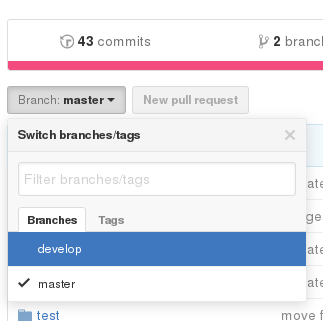
\includegraphics[width=0.3\linewidth]{github_branchList.png}}
    \hspace{3em}
    \subcaptionbox
        {GitHub 標籤列表。
        \label{fig:github_tagList}}
        {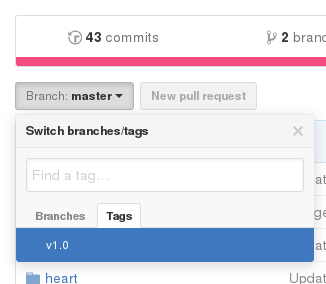
\includegraphics[width=0.3\linewidth]{github_tagList.png}}
    \caption{GitHub的分支及標籤列表。}
    \label{fig:github_branch_tagList}
\end{figure}

\subsection{專案結構}
\label{sec:s_template_structure}
專案根目錄包含教學(LaTeX tutorial)、各校規定(info)、各校樣板與語系(NCU\_zh)三類型目錄。另附上教學與樣板的編譯結果(*.pdf)作為閱讀以及對照使用者編譯之用。
各\LaTeX\ 目錄中的共用檔案及目錄(結尾含``/''者)如\cref{tab:template_structure} ,請盡量不要修改檔名或刪除檔案,除非你確定知道你在做什麼。
\let\tnote\tptabletnote
\begin{table}
    \centering
    \begin{threeparttable}
    \begin{tabularx}{\textwidth}{| l | X |}
        \hline
        codes/  & 用來存放程式碼。 \\ \hline
        figures/    & 用來存放論文中的圖片。亦可直接存在根目錄,但可能顯得凌亂。 \\ \hline
        NCU\_thesis.cls & 樣板連結,基本上不處理設定,提供各.tex子檔使用。 \\ \hline
        NCU\_thesis\_*.cls & 樣板主要設定,基於 extbook class,須要修改格式可以由此檔修改。 \\ \hline
        sppmgTools.sty & sppmg 提供的工具,可於各樣板間共用,因此另外獨立於cls。(請置於主檔同目錄或 \TeX\ 之套件搜尋路徑中) \\ \hline
        sppmgTools.cwl & sppmg 提供工具的指令形式,用於編輯器「自動完成」之功能(見\cref{sec:s_autocomplete}),請自行確認編輯器如何載入。 \\ \hline
        main.tex & 主檔案。\textbf{欲生成整份文件請編譯此檔}。檔案用於定義各子檔(章節)順序。  \\ \hline
        config.tex & 個人資訊設定檔。設定如論文題目等設定。\textbf{請設定使用之中文字型再編譯}。修改的方法是直接將花括號\{\}內改成你要的設定值\tnote{a},不然可能因找不中文字型而出錯。\textbf{本樣板可以利用設定作業系統來使用各系統預設字型}。  \\ \hline
        macros\_preamble.tex & 共用導言檔。將你要放在各個檔案導言區\tnote{b}的指令置於此檔。此檔將由NCU\_thesis.cls讀入,子文件中不須再引入。  \\ \hline
        macros\_document.tex & 共用文內設定。有些指令必須置於文內(\textbackslash{}begin\{document\}內),如設定字體大小的fontsize指令。這類型指令可置於此檔保持各子檔整潔以及避免漏放指令。(這個檔案會自動載入於\textbackslash{}begin\{document\}之後)  \\ \hline
        titlepage*.tex & 書名頁/封面,中央格式一樣,因此電子檔僅使用一張。(英文版有兩種封面,但如非必要建議僅用中文封面)  \\ \hline
        acknowledgements.tex & 誌謝(可不加,自行於main.tex註解掉。)  \\ \hline
        abbreviation.tex & 符號表。這裡簡單的以表格列出。\tnote{c}  \\ \hline
        abstract\_*.tex & 各語系摘要。  \\ \hline
        chapter\_*.tex & 各章節。(通常一章就一個檔。當然你可以再細分成更小的section子檔。\tnote{d}有些人會將chapter放在獨立目錄中,但以我的經驗,在搭配standalone等套件做子檔單獨編譯的情況下容易搞混相對路徑,所以我都放一起。)  \\ \hline
        appendix\_*.tex & 各附錄。  \\ \hline
        letter\_*.pdf & 各校須附文件。(不附加直接刪除即可,可不註解)  \\ \hline
    \end{tabularx}
    
    \caption{樣板目錄結構。}
    \label{tab:template_structure}
    
    \begin{tablenotes}
        \footnotesize
        \item[a]{儘量設定字型的英文名稱以避免出錯。Linux中可以使用指令``fc-list :lang=zh''來查詢可用的中文字型名稱。}
        \item[b] 何謂導言區,請見\cref{sec:s_latexDoc_structure}。
        \item[c] \LaTeX\ 亦有專用套件幫助處理術語,好處是可以自動進行排序,google關鍵字:Nomenclature(套件:nomencl)、Glossary(套件:glossary)以及綜合功能的套件:glossaries
        \item[d] 似乎在巢狀引入子擋上import套件比較好,請自行查閱說明手冊。
    \end{tablenotes}
    \end{threeparttable}
\end{table}
共用檔名開頭(如chapter\_*.tex)只是我個人為了文件目錄的整潔而自訂的規則,各位自行決定是否跟隨。

\chapter{\LaTeX\ 基礎教學}
\label{sec:c_basicLatex}
這裡的教學目的只是希望\LaTeX\ 新手可以無痛寫論文。所以只說明搭配此樣版後須要具備的基礎知識。如何調整樣板不是主要目標,有興趣或是有此需求的可以直接看\LaTeX\  code,內有一些註解或網頁連結可能可以幫到你。下面的說明我儘量以範例呈現,各位可以直接複製所須的\LaTeX\ 片段貼上論文再改。不過由pdf複製文字的部份怪怪的,可能要由\LaTeX\  原始碼複製。這部份可能是pdf cmap 等等的問題。

\section{背景知識}

\subsection{\TeX\ 、\LaTeX\ 歷史}
\LaTeX\  是一個非常強大、專業的排版軟體。事實上\LaTeX\ 其實是\TeX\ 的巨集。它使得原本較為困難的TeX語法變得簡單許多。
\TeX\  是 Donald Knuth 1977年為其巨著「The Art of Computer Programming」
\footnote{這本「神書」目前還沒寫完全套,希望Knuth有生之年可以順利完成。}
進行校稿時,發現當時的數學公式排版過於差勁,於是決定自己弄一個排版系統出來(這才是真正的Hacker !!)。由於直接寫\TeX\ (或稱Plain \TeX\ )文件較困難,因此後來發展出\LaTeX\ 來簡化上手難度。而後來又因為非英語、直接產生PDF 等等需求又衍生出各式各樣的\TeX\ /\LaTeX\ 版本。
\footnote{\TeX\  追求穩定,所以只除錯,不添加新功能。}

\subsection{編譯/生成PDF檔}
\LaTeX\  不同於LibreOffice Writer/ MS Office Word 之類的程式,它須要寫好tex檔之後以LaTeX程式(再透過Tex程式)編譯成最終檔案
\footnote{原始的\LaTeX\ 編譯器(就稱為latex)是將tex轉為dvi檔(可用evince等軟體開啟)。若要再轉pdf 須要再經由其他軟體轉換。}。% 編輯過程中無法看到排版結果,
其中tex檔為純文字檔,和常見的.txt 文字檔相同,亦即你可以由任何文字編輯器開啟,如Linux上的VIM或是Windows 上的記事本。相對的像是Word 的doc檔一定要用支援doc的程式才能開啟,否則會顯示成亂碼。

\LaTeX\  編譯器除了本身稱為\LaTeX\ 的程式外,尚有\XeLaTeX\ 、PdfLaTeX、LuaLaTex 等編譯器
\footnote{他們相對應的\TeX\ 編譯器分別是\XeTeX\ 、PdfTeX、LuaTex。事實上它們的特色是由*\TeX\  所提供而非*\LaTeX\ 。}
。其特色如下:
\begin{description}
    \item[XeLaTex]  支援Unicode 萬國字碼(原生UTF-8)。支援現代系統中的常見字型格式,如TrueType/OpenType,也就是說不須要另外載\LaTeX\  用的 PostScript 字型。輸出檔為PDF(但不支援DVI/PS)。
    \item[PdfLaTeX] 非Unicode,輸出檔為PDF。中文字碼處理須透過CJK套件,似乎以奇怪方式支援\footnote{\url{https://www.csie.ntu.edu.tw/~tzhuan/www/resources/ntu/}}。(其他優點我就不知啦!)
    \item[LuaLaTex] 人如其名;LuaLaTeX 即是基於 PdfLaTeX 再加上Lua 腳本引擎。由於 \TeX\  並不是真正的程式語言,要實現某些程式化動作可能須要拐彎抹角甚至是無法達成。而加上Lua則能夠以真正的程式語言優美的完成所須動作。支援Unicode 萬國字碼。
\end{description}
目前看起來\XeLaTeX\ 是較為先進與穩定的編譯器,因此本文僅針對 \XeLaTeX\  說明以及測試。(教學部份一般適用於所有\LaTeX\  編譯器,若你使用其他編譯器應該也只有少數區域要修改。)

\LaTeX\ 編譯時不會一次完成所有的工作,因此須要多次編譯。下面是含.bib文獻的標準編譯順序
\footnote{若須生成目錄(樣板main.tex會生成目錄),\textbackslash{}tableofcontents指令,須編譯到第二次才會生成。}
。(main表示main.tex,為某一專案的主檔案)
\begin{enumerate}
	\item xelatex main   $\longleftarrow$ 先編譯一次,部份內容如文獻以代號紀錄下來。
	\item biber main     $\longleftarrow$ 處理.bib文獻資料庫。biber 是BibLaTeX用的程式,若你用BibTeX則為 bibtex main
	\item xelatex main   $\longleftarrow$ 將上次編譯產生的代號替換為最終格式。
	\item (xelatex main) $\longleftarrow$ 可能視情況還須要更多次編譯(如makeindex)。
\end{enumerate}
通常\LaTeX\ 專用編輯器已經幫你處理好了,你只須要按下快速鍵(或圖示)一次就可以編譯完成。

指令介面的使用者對於單次編譯可以使用下面指令
\begin{lstlisting}[style=consoleStyle,language=bash]
xelatex -interaction=nonstopmode main
\end{lstlisting}

而多次編譯的話可以安裝latexmk 這個軟體,它可以自動完成所須的編譯動作。

\XeLaTeX\ 使用者推薦使用以下指令:\\
\begin{lstlisting}[style=consoleStyle,language=bash]
latexmk -xelatex -interaction=errorstopmode main
\end{lstlisting}
其中``-xelatex'' 指定用xelatex處理,須要latexmk 4.31版(2012年發佈)以上才可用。``errorstopmode''設定僅當編譯出錯才暫停,對於一些警告直接略過(時常因字體大小等等問題出現一堆警告,不理不會有任何問題)。亦可用nonstopmode取代之,但不甚推薦。
下面是某次我在 TeX Live 2016 上使用latexmk編譯後,輸出訊息結尾(首行\$表示Linux下輸入指令):
\begin{lstlisting}[style=consoleStyle,language=bash]
$ latexmk -time -xelatex -interaction=errorstopmode main
....
....
....
Output written on main.pdf (89 pages).
SyncTeX written on main.synctex.gz.
Transcript written on main.log.
Latexmk: Found input bbl file 'main.bbl'
Latexmk: Log file says output to 'main.pdf'
Latexmk: Found biber source file(s) [main.bcf tutorial.bib]
Latexmk: All targets (main.pdf) are up-to-date
'xelatex  -interaction=errorstopmode -recorder  "main.tex"': time = 5.92
'biber  "main"': time = 0.66
'xelatex  -interaction=errorstopmode -recorder  "main.tex"': time = 18.36
'biber  "main"': time = 0.920000000000002
'xelatex  -interaction=errorstopmode -recorder  "main.tex"': time = 18.01
'xelatex  -interaction=errorstopmode -recorder  "main.tex"': time = 18.2
'xelatex  -interaction=errorstopmode -recorder  "main.tex"': time = 18.09
Accumulated processing time = 82.53
\end{lstlisting}
會發現xelatex 總共執行5次。實際上次數不固定,所以若使用手動指定編譯次數方法,最好在編譯後檢視訊息,你可能會看到要求再次執行 biber 的訊息:
\begin{lstlisting}[style=consoleStyle,language=bash]
Package biblatex Warning: Please (re)run Biber on the file:
(biblatex)                main
(biblatex)                and rerun LaTeX afterwards.

 )
\end{lstlisting}
或是編譯完發現pdf檔缺東缺西(目錄不正常啦、todonotes 的線沒對到之類的)就可能要再執行一次 xelatex。

編譯過程中若是遇到錯誤會暫停,並顯示在終端上(假設你用文字式終端編譯以及使用了errorstopmode)。按<Enter> 鍵可以略過這個錯誤(文件也不會是完整的)。若是要直接終止編譯過程,可以輸入``x''。

編譯完成後,若你的系統上有Ghostscript (Linux上應該很常見)可以以下面指令壓縮pdf檔:
\begin{lstlisting}[style=consoleStyle,language=bash]
gs -dBATCH -dNOPAUSE -q -sDEVICE=pdfwrite -sOutputFile="Compressed.pdf" "Original.pdf"
\end{lstlisting}
壓縮後體積可以縮小不少,以我的論文來說縮了約40\%。不過缺點是pdf檔的附加資訊會連帶被消除。解決辦法是搭配pdftk取出附加資訊,gs處理完再匯入。
\footnote{\url{http://unix.stackexchange.com/questions/50475/how-to-make-ghostscript-not-wipe-pdf-metadata} 提到這是gs的bug,要利用pdftk處理。}

你可能會發現在編譯之後,工作目錄下出現許多奇怪附檔名的檔案。這是由於\LaTeX\  編譯時無法往回處理之前的標記,所以須要將標記資料紀錄下,待下次編譯時再處理。你可以不理會它們,對你而只有.tex(文件檔)、.bib(你置入的文獻資料庫)以及編譯生成的.pdf須要保留。不過有時會因為殘留的紀錄檔導致編譯出錯,所以有時遇到奇怪問題時記得試試先清除它們再編譯,或是直接將「清除紀錄檔」這個動作加到編譯序列的最前面。
\footnote{各檔案說明見\url{https://en.wikibooks.org/wiki/LaTeX/Basics\#Ancillary_files} }

\section{文件結構}
\label{sec:s_latexDoc_structure}
最簡單的\LaTeX\  文件如下:
\begin{lstlisting}[linewidth=0.9\textwidth]
\documentclass{article}
% This is comment, here is preamble.
\begin{document}
Hello world!
\end{document}
\end{lstlisting}
以\textbackslash{} 開頭的均為指令,而\{\}為其選項。
\textbackslash{}doocumentclass 選擇文件的類型(class),article 適合一篇簡單的文件(如實驗報告)。而其他如book/report則適合較大型的書、期刊等等。
不同的類型會產生不同風格的文件,如單雙面、單雙欄、頁眉頁尾、目錄等等。甚至連可使用的指令都有差異。選擇合適的類型可以省下很多調整的功夫。由於論文比較近似書的風格,因此本樣板即是使用(類)book class。
\footnote{說(類)是因為原始的book class 有字大小的限制,因此後來改用其他套件提供的book class。}
\textbackslash{}begin~\textbackslash{}end 則是某個環境的範圍。(這裡是document環境)\textbackslash{}begin\{document\} 表示其中為文件內容。而\textbackslash{}begin\{document\}前面的區域為導言區(preamble),用來設定所用的套件。

各個不同的文件的類型(class)提供不同的風格設定。以本樣板用到的book為例,其原始結構如下:
\begin{lstlisting}
\begin{document}
\frontmatter

\maketitle % print titlepage or cover
\tableofcontents		% table of contents (目錄)
\listoffigures			% list of figures (圖片列表)
\listoftables

% Introductory chapters
\chapter{Preface}
% ...

\mainmatter
\chapter{First chapter}
% ...

\appendix
\chapter{First Appendix}

\backmatter
\chapter{Last note}
\printbibliography % print bibliography in here.(文獻)
\end{document}
\end{lstlisting}
各區段(frontmatter/mainmatter/backmatter/...)有不同設定,如頁碼的差異、章節的編號等等。\textbackslash{}chapter 表示新的一章。類似的像是\textbackslash{}section、\textbackslash{}subsection 表示節、小節。
\footnote{樣板預設目錄顯示至第三級(\textbackslash{}subsection\{\}),章節編號標至第五級(\textbackslash{}paragraph\{\})。}


依照中央大學的要求,\textbackslash{}appendix 必須在\textbackslash{}backmatter後面
\footnote{據說APA格式亦要求\textbackslash{}appendix放至最後。}
,因此NCU樣板有對\textbackslash{}appendix做一點小小修改,使其置於\textbackslash{}backmatter 之後亦正常顯示。


\section{套件與指令}
\label{sec:s_basicCmd}
\LaTeX\ 文件中,提供各種特別功能的就稱為指令,而指令有些須要另載入「套件」才會有。譬如要打出水的化學式\ce{H_2O},你須要載入mhchem套件
\footnote{我知道有些人是直接用數學模式啦!}
,然後利用它提供的指令:\textbackslash{}ce\{H\_2O\}。

要載入套件可於導言區(preamble)使用:
\begin{lstlisting}
\usepackage[option]{package}
\end{lstlisting}

而各指令的形式如下
\begin{lstlisting}
\commandname[option1,option2, ...]{argument1}{argument2} ...
\end{lstlisting}
指令起始於\textbackslash{}。有些指令不帶參數,如\textbackslash{}LaTeX
% ,記得在結尾加上空格或是\{\}做結尾
\footnote{\textbackslash{}LaTeX用在文字行時,結尾要加上反斜線、空格:``\textbackslash{}LaTeX\textbackslash{}\ ''不然會和後面黏在一起。}
。
有些指令則是須要一個以上的參數,其中\{argument\}為必要參數。[option]為可略選項。譬如圖片說明文字的指令為: \\
\begin{lstlisting}
\caption[short]{full}
\end{lstlisting}
當填入[short]時,圖列表處的說明會換成短版的說明(顯示於圖目錄)。

\textbackslash{}起始的指令名稱直到空格或保留字才結束,因此對於內文中的無參數指令一定要加空格或是以\{\}結束。下面示範於內文中(以text夾住)使用指令
\begin{table}[h]
    \centering
    \caption{指令範例}
    \begin{tabular}{| l | l |}
        \hline
        \verb*|text\cmd text|  & o  Valid \\ \hline
        \verb*|text\cmd{}text| & o  Valid \\ \hline
        \verb*|text\cmdtext|   & x  Invalid \\ \hline
        \verb*|text\cmd文字|    & x  Invalid \\ \hline
    \end{tabular}
\end{table}


有些指令提供帶星號形式。如\textbackslash{}chapter 與\textbackslash{}chapter$\ast$ ,後者將產生一個無編號的章節,同時也不顯示於目錄。

指令的參數([]或是\{\})內不能有多餘的空格。譬如插入圖片時的路徑若在結尾多打一個空格:
\begin{lstlisting}[showspaces=true]

\includegraphics{logo-Linux.png }
\end{lstlisting}
編譯時會出現錯誤,因為編譯器會將空格視為檔名,所以找不到檔案。

\section{文字}
\label{sec:s_text}
\LaTeX\  中的文字編排有以下特性:
\begin{itemize}
    \item 除了保留字外,一般文字直接打就可以顯示在文件上。
    \item 區分大小寫。\textbackslash{}chapter 與 \textbackslash{}Chapter 是不一樣的。
    \item 縮減空格。文字間多個空格與單一空格等效,僅會顯示出同樣的間隔,而此一間隔由\LaTeX\  編譯器判斷。
    \item 忽略單一斷行。單一斷行與連接在一起是等效的。二個以上的斷行視為新的段落。若要強制斷行但不分段可以使用雙反斜線:\textbackslash{}\textbackslash{}。
    \item 英文``引號'',左邊要用兩個「\verb|`|」(曲線號「$\sim$」那顆鍵,1左邊),右邊要用兩個「\verb|'|」(Enter左邊的鍵)
\end{itemize}


\subsection{保留字}
以下字元為保留字,直接使用不會出現在文件上(大部分會導致編譯失敗)。 
\begin{table}[h]
    \centering
    \begin{tabular}{|l|l|l|}
    \hline
    保留字 &            顯示文字指令         & 保留字功能 \\ \hline
    \#  &              \textbackslash{}\#  & 定義指令的選項 \\ \hline
    \$  &              \textbackslash{}\$ & 數學模式標記 \\ \hline
    \%  &              \textbackslash{}\% & 註解 \\ \hline
    \^{}    &          \textbackslash{}\^{}\{\} & 上標,用於數學模式\\ \hline
    \&  &              \textbackslash{}\& & 矩陣、表格分隔符 \\ \hline
    \_  &              \textbackslash{}\_ & 下標,用於數學模式\\ \hline
    \{  &              \textbackslash{}\{ & 指令參數標記\\ \hline
    \}  &              \textbackslash{}\} & 指令參數標記\\ \hline
    \~{}    &          \textbackslash{}\~{}\{\} &\\ \hline
    \textbackslash{} & \textbackslash{}textbackslash\{\}& 指令起始字元\\ \hline
    \end{tabular} 
\end{table}


\subsection{字體大小與行高}
{\color{red}
本樣板已提供豐富、簡便的「字體大小與行高」設定,請於config.tex中「字體大小風格及行距」、「標題風格」等選項設定。直接使用\LaTeX\ 指令即可。風格均可疊加,如``\textbackslash{}sffamily\textbackslash{}Large''。
}

\subsubsection{字體大小}
\LaTeX\ 中的字體大小基本上使用相對大小的方式設置。在一開始載入class 檔時就先決定基礎字體大小。之後文內(以及標題等等)使用相對大小進行修改,如\textbackslash{}large、\textbackslash{}small。
\footnote{其對應的真實大小可以由wikibook查到,也可以自己寫指令測量。}
此外,我們也可以經由anyfontsize套件提供的\textbackslash{}fontsize指令來調整字的絕對大小。

設定基礎大小的方法如下:
\begin{lstlisting}
\documentclass[a4paper,10pt]{book}
\end{lstlisting}
10pt(1pt=1/72.27 inch
\footnote{\TeX\ 中pt 定義和 Adobe 的 PostScript pt不同,Adobe 的pt在 \TeX\ 中稱為bp,1bp=1/72 inch。Word似乎也是以bp做單位。}
)即為這個例子所設定的大小(事實上10pt也是book class預設值,不指定就是10pt)。不過10pt對於中文來說太小,而\LaTeX\ 預設文件類別又只提供有限的選項(10pt,11pt,12pt)。
若要用更大的字體,解決方法有兩種。一是改用其他套件提供的class,另一是在內文區段(\textbackslash{}begin\{document\}內)使用\textbackslash{}fontsize調整。

改用其他套件提供的class方面。如extsize套件對應的extbook class提供了 8pt, 9pt, 10pt, 11pt, 12pt, 14pt, 17pt, 20pt這些選項。而 KOMA-script的scrbook class則是使用無級縮放[fontsize=14pt]。
由於本樣板目前(v1.6)採用extsize,所以請從extbook class的大小選項中選一個使用並填入main.tex的\textbackslash{}documentclass選項(樣板預設中文樣板使用14pt,英文使用12pt)。
設定範例如下:(documentclass使用extbook舉例,樣板使用者請維持原本的documentclass。)
\begin{lstlisting}
\documentclass[a4paper,10pt]{extbook}
\end{lstlisting}

若是採用\textbackslash{}fontsize調整文字,雖然它可以方便的無級縮放文字,但要注意
\textbackslash{}fontsize只能放在\textbackslash{}begin\{document\}內(樣板提供macro\_document.tex,置於此即可),並且只能暫時影響其後的文字。當遇到\textbackslash{}large之類的指令時將調回基礎大小的「large大小」(以及行高),有可能發生\textbackslash{}large比原文還小的情況。
\textbackslash{}fontsize範例如下:
\begin{lstlisting}
% \fontsize{size}{baselineskip}\selectfont
\fontsize{10}{12}\selectfont 
\end{lstlisting}
size指定大小(單位pt),baselineskip為行高(\LaTeX\ 預設值10pt,12pt。(一倍行高=1.2x))。

相對的修改字體大小指令示範如\cref{tab:fontsize}
\footnote{完整列表見wikibook:\url{https://en.wikibooks.org/wiki/LaTeX/Fonts\#Sizing_text}}
:
\begin{table}[h]
    \centering
    \caption{字體大小範例(指令前後的\{\}作用為限制影響範圍)}
    \begin{tabular}{| l | l |}
        \hline
        指令                                & 效果         \\ \hline
        \{\textbackslash{}tiny ...\}        & {\tiny 字體大小}\\ \hline
        \{\textbackslash{}footnotesize ...\}       & {\footnotesize 字體大小} \\ \hline
        \{\textbackslash{}small ...\}       & {\small 字體大小} \\ \hline
        \{\textbackslash{}normalsize ...\}  & {\normalsize 字體大小} \\ \hline
        \{\textbackslash{}large ...\}       & {\large 字體大小} \\ \hline
        \{\textbackslash{}LARGE ...\}       & {\LARGE 字體大小} \\ \hline
        \{\textbackslash{}Huge ...\}        & {\Huge 字體大小} \\ \hline
    \end{tabular}
    \label{tab:fontsize}
\end{table}
再次提醒!所有的大小都是相對於\textbackslash{}normalsize而訂,而這個\textbackslash{}normalsize就是一開始傳給class的數值。

本樣板於1.5版以前採用\textbackslash{}fontsize,1.6版後已經遷移至extbook,所以預設不用\textbackslash{}fontsize做調整。不過仍舊於 macro\_document.tex保留註解掉的\textbackslash{}fontsize。
更豐富的字體大小設定請見\url{http://texblog.org/2012/08/29/changing-the-font-size-in-latex/}

\subsubsection{行高}
行高方面有多種設定方式。(\textbackslash{}fontsize可以直接設定,這裡就不再提了)
本樣板採用的方式是利用setspace套件設定。
\begin{lstlisting}
\setstretch{1.5} 
\end{lstlisting}
上面的設定將使得行高變更為1.5倍,這也是公認最舒適的行距並且是本樣板預設值。不過表格內容以及caption也會因此而改成1.5倍,不太好看。沒關係!本樣板已經幫你調好,只要在config.tex中分別設定即可。(細節我就不講啦!自己去研究cls檔。)

其他不用套件調行高的方法如下:
\begin{lstlisting}
\renewcommand{\baselinestretch}{1.5} 
\end{lstlisting}
免套件,但統一調整所有行距。彈性不如setspace套件。
\begin{lstlisting}
\linespread{1.3} 
\end{lstlisting}
倍數不直觀,例如1.6為2倍行高。

\subsection{字型樣式}
\LaTeX\ 中的字形樣式以指令設定,包含文字風格(粗、斜體)以及字型。下面這張表格示範了常用的樣式指令以及效果。其中第一欄(\LaTeX\ )指令會影響後面的所有文字
\footnote{可使用\{\}來限制範圍,如\{\textbackslash{}em ... \}}
。第二欄(小範圍)則是只影響\{...\}中的內容。最後面分別測試中英文的效果。
\footnote{改自\LaTeX\  wikibook:\url{https://en.wikibooks.org/wiki/LaTeX/Fonts\#Shapes}}
\footnote{底線須要另外使用ulem套件,理由是應以emphasis取代,見wikibook。中文的xeCJK亦支援ulem套件,請參考其手冊。}
\begin{table}[h]
    \centering
    \caption{樣式範例}
    \begin{tabular}{| l | l | l |}
        \hline
        \LaTeX\        &  小範圍   &  效果 \\ \hline
        \textbackslash{}normalfont  & \textbackslash{}textnormal\{...\}   & \textnormal{正常normal} \\ \hline
        \textbackslash{}em          & \textbackslash{}emph\{...\}         & \emph{強調emphasis} \\ \hline
        \textbackslash{}rmfamily    & \textbackslash{}textrm\{...\}       & \textrm{羅馬(襯線)roman}\\ \hline
        \textbackslash{}sffamily    & \textbackslash{}textsf\{...\}       & \textsf{無襯線sans serif}\\ \hline
        \textbackslash{}ttfamily    & \textbackslash{}texttt\{...\}       & \texttt{打字機(等寬)teletypefont(monospace)}\\ \hline
        \textbackslash{}bfseries    & \textbackslash{}textbf\{...\}       & \textbf{粗體bold}\\ \hline
        \textbackslash{}itshape     & \textbackslash{}textit\{...\}       & \textit{斜體italic}\\ \hline
    \end{tabular}
\end{table}
本樣板中,\textbackslash{}rmfamily, \textbackslash{}sffamily, \textbackslash{}ttfamily 可以由config.tex的 \textbackslash{}def\textbackslash{}mainfont等指令設定使用的字型,中文則是\textbackslash{}def\textbackslash{}CJKmainfont等指令。
\footnote{事實上是透過 fontspec套件提供的 \textbackslash{}setmainfont, \textbackslash{}setsansfont, \textbackslash{}setmonofont進行設定。而對應的中文則是由xeCJK套件提供的\textbackslash{}setCJKmainfont,\textbackslash{}setCJKsansfont,\textbackslash{}setCJKmonofont }

普通文件常用的字體有\textsf{楷體}以及明體(或用宋體)兩種。通常內文較適合細字的明體,這樣讀起來較不容易疲勞。而楷體適合放在字體、空間較大的標題,因此本樣板中設定中文的主要字體為明體,而無襯線字體則是設定楷體
\footnote{若要在一段文字中暫時的使用襯線英文與楷體,可以簡單的用\textbackslash{}rmfamily\textbackslash{}CJKfamily{sf}達成,見\cref{sec:s_fonts}。}
。若要新增其他字型,可以使用\textbackslash{}newfontfamily來設定。下面是一個簡單的範例,這裡假設你的系統中有「cwTeX 楷書」字型。
\begin{lstlisting}[style=LatexStyle,xleftmargin=0.5cm]
\begin{document}
\newfontfamily\cwbm{cwTeX 楷書}
正常文字
{\cwbm 使用cwTeX楷書}
正常文字
\end{document}
\end{lstlisting}

有些文件會以一種較短的指令來設定樣式,如粗體使用\textbackslash{}bf、斜體使用 \textbackslash{}it。這是舊的指令,存在某些問題。現在(2016年)請用\textbackslash{}bfseries、 \textbackslash{}itshape。

\section{圖片}
\label{sec:s_figure}
\XeLaTeX\ 支援的圖片格式有eps, pdf, png, jpg。數據圖推薦使用eps格式,因為eps是向量圖檔,縮放不會失真。流程圖或一些手繪線條圖,雖然\LaTeX\ 有套件可以畫出,但我建議初學者還是用Dia/LibreOffice Draw之類的,先畫完再匯出成eps插入比較快。
\footnote{推薦的自由軟體:影像、照片修圖:GIMP。向量圖、手繪線條:Inkscape、LibreOffice Draw。流程圖/關係圖:Dia、Graphviz}
LibreOffice Draw的匯出方法見\cref{sec:a_loDraw}。
\footnote{M\$ Office 「力點」據說無法匯出成eps格式。}

這裡用的圖片全部都不採用「文繞圖」模式,一般正式文件應該也很少使用文繞圖。欲使用的話可使用wrapfigure套件。
\footnote{\url{https://nl.sharelatex.com/learn/Inserting\_Images}}

\subsection{插入單一圖片}
\begin{LTXexample}[style=LatexStyle,xleftmargin=0.5cm]
\begin{figure}[!htb]
    \centering
    
\includegraphics[width=0.2\textwidth]{logo-Linux.png}
    \caption[Linux logo]{This is a Linux logo. It is a penguin.}
    \label{fig:first_linux_logo}
\end{figure}
\end{LTXexample}
注意幾件事:
\begin{itemize}
    \item \{figure\}環境為一個浮動性環境,也就是說在沒有使用[h]選項的情況下,\LaTeX\ 會自動為我們選擇適當位置。細節請參考\cref{sec:s_float}
        \footnote{本樣板已於cls中設定FloatBarrier,浮動環境不會超出\textbackslash{}subsubsection範圍。}
    \item \textbackslash{}includegraphics中,width=0.2\textbackslash{}textwidth 指得是縮放圖形至0.2倍行寬。
    \item \textbackslash{}label須要放在\textbackslash{}caption之後,因為\textbackslash{}caption存在\textbackslash{}label才會生成標記。
\end{itemize}
若只是插入一張圖片,上面的指令稍嫌麻煩,於是我提供一個簡化指令,其語法如下:
\begin{lstlisting}
\fig[scalefactor][fig:label][!htb]{path}[caption][short caption]
\end{lstlisting}
除path外,其餘均可忽略,但須注意[]在\{\}前後分別為前三後二,若提供數目不足會當作左方的設定值。例如\{\}前只提供兩個[],則第一個為[scalefactor],第二個為[fig:label]
\footnote{雖然這裡寫得是[fig:label],但其實``fig:'' 就是 label 的內容,見\cref{sec:s_labelRef}。}
。若須要忽略中間的[fig:label]必須補上空括號,以下照優先順序排列說明。
\footnote{[scalefactor]基於\textbackslash{}textwidth,也就是文字行寬。數值範圍[0~1]}
\begin{enumerate}
    \item path,圖片路徑含副檔名。
    \item scalefactor縮放因子,0.0~1.0倍行寬,預設0.5
    \item label標籤,省略則預設「fig:」+ 檔名(path)
    \item !htb浮動選項,預設為空,即交由\LaTeX\ 排版。
    \item caption,圖片說明,顯示在\textbackslash{}includegraphics的相對位置。
    \item short caption短圖說,用來取代圖目錄裡的文字,預設為空,即同caption。
\end{enumerate}
須要注意的是括號僅path為大/花括號,這是因為路徑為必要參數。以下示範各種使用方法:
\begin{LTXexample}[style=LatexStyle,xleftmargin=0.5cm]
\fig{logo-Linux.png}
\fig{logo-Linux.png}[line 2, caption]
\fig[0.15]{logo-Linux.png}
\fig[0.15][][h]{logo-Linux.png}[line 4, caption]
\fig[0.15][fig:label_test_1][h]{logo-Linux.png}[line 5, caption]
\fig[0.15][fig:label_test_2]{logo-Linux.png}[line 6, caption]
\fig[0.15][fig:label_test_3][!hbt]{logo-Linux.png}[line 7, caption][short caption]
\end{LTXexample}
省略label的圖會自動設定label為``fig:logo-Linux.png''

\subsection{插入多張圖片}
這裡使用subcaption套件並且使用\textbackslash{}subcaptionbox ,它可以對齊各子圖的底部,多行caption時比較整齊。下面範例同時示範文內引用的方法。
\begin{LTXexample}[style=LatexStyle,xleftmargin=0.5cm,preset=\let\label\orilabel]
\begin{figure}[!hbt]
    %\captionsetup[subfigure]{labelformat=empty} % 完全隱藏圖號
    \centering
    \subcaptionbox
        {Linux (A kernel of OS)
        \label{fig:subfig_linux}}
        {
\includegraphics[width=0.3\linewidth]{logo-Linux.png}}
    ~
    \subcaptionbox
        {Debain (A popular distribution). Demo long caption,  bla bla bla bla bla.
        \label{fig:subfig_debian}}
        {
\includegraphics[width=0.3\linewidth]{logo-Debian.eps}}
    \vspace{\baselineskip} % 分隔上下列
    \subcaptionbox
        {GNU (A project of OS)
        \label{fig:subfig_gnu}}
        {
\includegraphics[width=0.6\linewidth]{logo-GNU.png}}
     % use ``\subref{fig:subfig_debian}'' get ID of subfigure(this ID is Debian)
    \caption{caption, 這裡可使用 \subref{fig:subfig_debian}取得子圖(Debian)編號 }
    \label{fig:multifig_label}
\end{figure}
% 以下內文示範引用
\cref{fig:multifig_label}為三張圖的編號,Debian是\cref{fig:subfig_debian}。
\end{LTXexample}
``\~{}'' 表示在圖片間插入間隔,當圖片較密時比較美觀(亦可用\textbackslash{}hspace\{\}來指定)。圖片一行的寬度總和建議不要超過「0.98\textbackslash{}linewidth」,不然會自動折行跑到下一行去。
若要控制圖片如「品」字排列(強制換行),可以將上面的``\~{}'' 取代為空行,若要再加大上下間距可以用\textbackslash{}vspace\{\}
\footnote{\textbackslash{}hspace\{\}、\textbackslash{}vspace\{\}可指定長度單位,如\textbackslash{}hspace\{5mm\}}
。
當子圖太小時, caption 可能會因為圖片不夠寬導致折行並加大文字間距,非常難看。可以加上subcaptionbox的寬度選項,如: \textbackslash{}subcaptionbox\{caption\}[5cm]\{\textbackslash{}includegraphics .... \} 手動設定圖框的寬度。
如果要做其他更細緻的子圖位置設定,請自行參考minipage用法。
\footnote{\url{http://tex.stackexchange.com/questions/55337/how-to-use-figure-inside-a-minipage}}

引用子圖時直接使用子圖(\textbackslash{}subcaptionbox)的\textbackslash{}label的標記即可,子圖會自動加上編號。


\section{表格}
\label{sec:s_table}
表格如果太複雜不會製作或是嫌不好輸入,可以找圖形界面的軟體或是線上網站。同樣的,有些編輯器也已經內建表格產生器了,不過功能可能很陽春就是了。
表格的說明文字(caption)位置改設定在表格上方。(雖然說caption位置可以透過\textbackslash{}caption和tabular環境的相對位置來設定,但產生出的caption與表格距離會過近
\footnote{事實上這個距離由\textbackslash{}abovecaptionskip 和\textbackslash{}belowcaptionskip 設定,預設為10pt、0pt。}
,所以本樣板透過floatrow套件設定表格的caption位置,\LaTeX\ code 中\textbackslash{}caption也不必特別寫在tabular上方。)

表格的\{table\}環境和\{figure\}環境一樣屬於浮動性環境,詳情見\cref{sec:s_float}中的說明。
\subsection{一般表格}
\begin{LTXexample}[style=LatexStyle,xleftmargin=0.5cm]
\begin{table}[h]
    \centering
    \caption{Solution}
    \begin{tabular}{| l | l |}
        \hline
        Component & Concentration(mM) \\ \hline
        \ce{NaCl} & 118.0 \\ \hline
        \ce{CaCl_2} & 2.11 \\ \hline
        \ce{KCl} & 4.69 \\ \hline
    \end{tabular}
    \label{key}
\end{table}
\end{LTXexample}
\textbackslash{}begin\{tabular\}\{| l | l |\}旁的「|」表示畫垂直線,英文字母「l」表示左對齊,\textbackslash{}hline表示水平線。對齊控制除了「l」外,亦可用「c」(center)、「r」(right)。表格分隔若想用其他字元亦可用「@\{\}」處理,樣板的符號列表就是利用冒號分隔「@\{:\}」

\subsection{自動折行表格}
tabularx 套件的 tabularx 環境可以設定表格寬度,過長的內容將自動折行(其實這才是我的目的)。下面以原始tabular進行對照。當文字寬度超出表格時,原始tabular會超出頁面(下面超出的表格是正常的喔!),而tabularx會自動折行以及調整表格至行寬。
\footnote{更多資訊請參考wikibook https://en.wikibooks.org/wiki/LaTeX/Tables\#The\_tabularx\_package }

\begin{LTXexample}[style=LatexStyle,xleftmargin=0.5cm]
\begin{table}[h]
    \centering
    \begin{tabular}{| l | l |}
        \hline
        short & ssssssss \\ \hline
        long & llllllllll lllllll llllllll lllllllllll llllllll \\ \hline
    \end{tabular}
    \label{key}
\end{table}

\begin{table}[h]
    \centering
    \begin{tabularx}{\textwidth}{| l | X |}
        \hline
        short & ssssssss \\ \hline
        long & llllllllll lllllll llllllll lllllllllll llllllll \\ \hline
    \end{tabularx}
    \label{key}
\end{table}
\end{LTXexample}

\subsection{合併欄位表格}
示範合併欄位。
\begin{LTXexample}[style=LatexStyle,xleftmargin=0.5cm]
\begin{table}[h]
    \centering
    \begin{tabular}{| l | l | l | l |}
        \hline
        1 & 2 & 3 & d \\ \hline
        4 & 5 & \multirow{2}{*}{66} & e \\ 
        \cline{1-2}\cline{4-4}
        7 & 8 & & f  \\ \hline
        9 & \multicolumn{2}{c|}{ a }& g  \\ \hline
        b & c & h & i  \\ \hline
    \end{tabular}
    \label{key}
\end{table}
\end{LTXexample}

\subsection{其他表格}
\LaTeX\ 預設的tabular表格無法使用腳註(footnote),此外還有無法處理太長、太寬的表格等問題。須要用到的話可見\cref{sec:s_advTable}的說明。

\section{列表/條列}
\label{sec:s_list}
常用的列表形式有項目(itemize)、數字(enumerate)、描述(description)三種,以下示範項目(itemize)列表:
\begin{LTXexample}[style=LatexStyle,xleftmargin=0.5cm]
\begin{itemize}
    \item item 1
    \item item 2
    \begin{itemize}
        \item item 2.1 $\quad \leftarrow$ nesting
        \item item 2.2
    \end{itemize}
    \item item 3
\end{itemize}
\end{LTXexample}
列表允許巢狀使用,也就是在列表環境中再包一個列表。下面的示範就只列出兩個項目。\\
數字(enumerate)列表:
\begin{LTXexample}[style=LatexStyle,xleftmargin=0.5cm]
\begin{enumerate}
    \item item 1
    \item item 2
\end{enumerate}
\end{LTXexample}
描述(description)列表:
\begin{LTXexample}[style=LatexStyle,xleftmargin=0.5cm]
\begin{description}
    \item[description 1] item 1
    \item[description 2] item 2
\end{description}
\end{LTXexample}


\section{數學符號、方程}
\label{sec:s_math}
數學式的編輯實在太廣,這裡只講解一些基本概念。
更多資訊請參考wikibook: \url{https://en.wikibooks.org/wiki/LaTeX/Mathematics}

\subsection{顯示模式}
\LaTeX\ 中的常用數學顯示模式有下面三種:
\begin{itemize}
    \item Equation 環境,由\textbackslash{}begin\{equation\}...\textbackslash{}end\{equation\}包起來。數學式會獨立成行,並且擁有一個編號。
    \item Displaymath 環境 ,通常直接使用\textbackslash{}[...\textbackslash{}]包住數學式即可。數學式獨立成行但無編號。
    \item Inline math 環境。使用\$...\$包住數學式。數學式與普通文字同一行,並且字體一樣大。
\end{itemize}
下面分別示範這三種顯示模式。
\begin{LTXexample}[style=LatexStyle,xleftmargin=0.5cm]
\textbf{Equation, new line and numbered}\\
start equation
\begin{equation}
\oint_C {E \cdot d\ell} = 0
\end{equation}
end equation \\
------------------------\\
\textbf{Displaymath, new line} \\
start equation
\[
\oint_C {E \cdot d\ell} = 0
\]
end equation \\
------------------------\\
\textbf{Inline}\\
start equation
$\oint_C E \cdot d\ell = 0 $
end equation
\end{LTXexample}
以我的習慣來說,一律使用 Equation 環境,即使不一定用到編號。

\subsection{常用數學符號}
下面示範常用數學符號。(如果你用的是\LaTeX\ 專用編輯器,通常都有按紐可以輔助插入指令,不用拿個手冊在旁邊對照。)

\begin{table}[h]
    \centering
    \caption{常用數學符號}
    \begin{tabularx}{\textwidth}{| l | l | >{\raggedright\arraybackslash}X |}
        \hline
        \LaTeX\         & Result    &   說明      \\ \hline
        \verb|A_i=\mathrm{e}^{-x}|   & $A_i=\mathrm{e}^{-x}$        & \^{}\ \_{} 為上、下標。\textbackslash{}mathrm標示數學文字 \\ \hline
        \verb|(a+b-c)\cdot d \times e| & $(a+b-c)\cdot d \times e$  & 加、減、乘 \\ \hline
        \verb|\frac{\frac{1}{x}+^1/_{y}}{y-z}|&$\frac{\frac{1}{x}+^1/_{y}}{y-z}$ & 兩種除法 \\ \hline
        \verb|\cos^2 \theta - \sin^2 \theta| & $\cos^2 \theta - \sin^2 \theta$ & 三角函數\\ \hline
        \verb|\alpha\beta\gamma\Omega| & $\alpha\beta\gamma\Omega$ & 希臘字母 \\ \hline
        \verb|50\textbaht| & $50\textbaht$ & 一隻喬巴 (須要textcomp套件)\\ \hline
        \verb|\infty| & $\infty$ & 富間 \\ \hline
    \end{tabularx}
\end{table}
數學模式中,非指令文字均視為變數,而變數一律以斜體表達。為了避免一些非變數文字變成斜體就必須特別處理。(載入amsmath套件後)\textbackslash{}text與\textbackslash{}mathrm就是處理這個問題。\textbackslash{}text通常用在純文字上,而\textbackslash{}mathrm則是符號類文字。
\footnote{\url{http://tex.stackexchange.com/questions/19502/is-there-a-preference-of-when-to-use-text-and-mathrm}}

\section{科學符號}
\label{sec:s_science}
這兩者雖然有時可用其他方法達成,譬如像溫度\temp{} , 有人會用圓圈加上C,有人用字碼。但基於排版以及可讀性我會建議各位用專用套件(\LaTeX\  style :D )。
\subsection{SI單位}
使用siunitx套件。一些常用的如溫度,我會另外寫指令加速完成。如何寫見後面章節說明。
\begin{LTXexample}[style=LatexStyle,xleftmargin=0.5cm]
$\SI{30}{\centi\metre}$ \\
$\SI{5}{\milli\litre}$ \\
$\SI{25}{\degreeCelsius}$ \\
\temp{37} <-- my command
\end{LTXexample}

\subsection{化學式}
前面表格已經示範了。使用到mhchem套件
\footnote{TeX Live 2016 的 mhchem為第四版,但我的TeX Live 2012的mhchem套件為第三版,所以我在cls檔中設定mhchem選項[version=3] ,如果各位沒有相容性問題又想用最新版可以取消掉。我保留這個設定也是怕說mhchem未來更動語法可能會出現論文移到新的TeX發行版後就不能用的情況。}
。表達離子帶電用\^{},原子數用\_ 。離子帶電可以不加上標,因為用在後面預設視為上標模式。
\begin{LTXexample}[style=LatexStyle,xleftmargin=0.5cm]
\begin{table}[h]
    \centering
    \begin{tabular}{| l | l |}
        \hline
        \ce{Ca2+} & x \\ \hline
        \ce{Ca^2+} & o \\ \hline
        \ce{Ca^{2+}} & o \\ \hline
    \end{tabular}
\end{table}
\end{LTXexample}

\section{標記與參考Cross-referencing}
\label{sec:s_labelRef}
「標記與參考」是\LaTeX\ 很好用的一個功能。各位千萬不要手打「見圖 1.1」啊!!標記可以設定一個標籤給它,而內文可以藉由參考指令取得標記位置的數值。這功能可以用在圖、表格、章節、文獻之上。

\subsection{標記(label)}
標記方法前面已經提到,用\textbackslash{}label\{type:mylabel\}標記。type方面如\cref{tab:label_type}所示。
\begin{table}[t]
    \centering
    \caption{常用標記類型}
    \begin{tabular}{| l | l |}
        \hline
        fig & figure \\ \hline
        tab & table \\ \hline
        eq  & equation \\ \hline
        sec & section \\ \hline
    \end{tabular}
    \label{tab:label_type}
\end{table}
有些套件會用到這個縮寫,所以最好符合通用習慣。(其餘見 \url{https://en.wikibooks.org/wiki/LaTeX/Labels_and_Cross-referencing\#Introduction})
稍微注意的是\textbackslash{}label\{\}要放在\textbackslash{}caption\{\}之後才會有作用。(caption也不能為空喔!)

\subsection{參考(ref/cref)}
假設你已經在figure中使用\textbackslash{}label\{fig:image001\},那文章中若要產生此圖的標號可以用\textbackslash{}ref\{fig:image001\},但有時我們懶得每個圖都要打``\emph{fig}. \textbackslash{}ref\{fig:image001\}這樣,所以我這使用了cleveref 套件。它提供\textbackslash{}cref指令自動產生相對應的文字。
\footnote{文字可以由\textbackslash{}crefname修改,見cls檔。cleveref亦提供大寫版\textbackslash{}Crefname用於行首風格(大寫)。不過中文無此須求。}
% \fig[0.3][fig:reftest0]{logo-Linux.png}[this is ref test figure.]
% (insfig will add ``fig:'')\\
% Use \textbackslash{}ref :\ref{fig:reftest}\\
% Use \textbackslash{}cref :\cref{fig:reftest}
\begin{LTXexample}[style=LatexStyle,preset=\let\label\orilabel]
\begin{figure}
    \centering
    
\includegraphics[width=0.2\textwidth]{logo-Linux.png}
    \caption[Linux logo]{This is a Linux logo. It is a penguin.}
    \label{fig:reftest}
\end{figure}

Use \textbackslash{}ref :\ref{fig:reftest}\\
Use \textbackslash{}cref :\cref{fig:reftest}
\end{LTXexample}
\textbackslash{}cref 支援多個標籤,如:\textbackslash{}cref\{ref1,ref2,ref4\} 。
\textbf{(注意!中間不可插入空格。)}
亦提供連續引用指令\textbackslash{}crefrange。
\footnote{範例見\url{http://texblog.org/2013/05/06/cleveref-a-clever-way-to-reference-in-latex/},連接文字、符號欲修改請參考手冊。}

\section{文獻}
\label{sec:s_bib}
如同之前的\textbackslash{}label、\textbackslash{}ref 。插入引用文獻須要建立文獻條目,再利用\textbackslash{}cite\{cite\_key\}來插入條目編號。
\footnote{下面提到的bibtex, biber, biblatex, natbib 詳細資訊可參考  \url{http://tex.stackexchange.com/questions/25701/bibtex-vs-biber-and-biblatex-vs-natbib}}

\subsection{嵌入式文獻資料庫}
少量條目時可以直接使用嵌入的方式,於thebibliography環境以 \textbackslash{}bibitem\{cite\_key\} 嵌入至tex檔中,然後以\textbackslash{}cite\{cite\_key\}插入文章。
\footnote{這裡因為示範生成檔會導致章節錯亂,所以只列出\LaTeX\ 碼。}
\begin{lstlisting}
\begin{thebibliography}{9}

\bibitem{lamport94}
  Leslie Lamport,
  \emph{\LaTeX\ : a document preparation system},
  Addison Wesley, Massachusetts,
  2nd edition,
  1994.

\end{thebibliography}
see bibliography \cite{lamport94}.
\end{lstlisting}
``lamport94'' 即為cite\_key 。而\textbackslash{}begin\{thebibliography\}\{9\} 的9指得是生成的條目上限為9條。據wikibook指出嵌入式的上限為99。

\subsection{BibTeX}
\begin{center}
\noindent{\color{red}\textbf{本樣板採用的是BibLaTeX,請見\cref{sec:s_bib_biblatex}。}}
\end{center}

針對大量文獻,通常使用文獻管理軟體先產生一個包含各條目的.bib檔(亦為純文字檔),再於tex中引入。
傳統上使用BibTeX這軟體,只要在要生成文獻地方插入\textbackslash{}bibliography\{Path\_of\_BibTeX\_database\}即可。
\begin{lstlisting}
\bibliographystyle{plain}
\bibliography{sample1,sample2,...,samplen} 
% Note the lack of whitespace between the commas and the next bib file.
\end{lstlisting}
這裡示範引入多個bib資料庫,也就是sampleN,注意中間不能有空格。若要使用與編譯文件不同目錄的資料庫,可以使用相對路徑表達,如``../sample1''。
\footnote{tex檔中的路徑一律使用正斜線``/'',即使是在windows中編譯。}
一開頭的\textbackslash{}bibliographystyle用途則是指定生成的風格。

用了BibTex之後,記得要再多執行一次編譯動作。也就是說要經過 xelatex tex $\rightarrow$ bibtex tex $\rightarrow$ xelatex tex 三個動作。tex附檔名(.tex)不用加。

BibTeX生成的文獻編號一律是數字,如果你須要更有變化譬如作者和年份(eg. Roberts, 2003),那你可以使用Natbib套件,不過\textbackslash{}cite指令須要修改。這部份請自行查詢wikibook
\footnote{\url{https://en.wikibooks.org/wiki/LaTeX/Bibliography_Management\#Natbib}}
\footnote{ShareLaTeX 有一個 BibTeX風格列表預覽 https://www.sharelatex.com/learn/Bibtex\_bibliography\_styles }
。

\subsection{BibLaTeX}
\label{sec:s_bib_biblatex}
另一個管理大量文獻的方法則是使用 BibLaTeX。雖然這裡說是「使用 BibLaTeX」,但實際上處理文獻資料庫的是biber這個程式。
\footnote{亦可使用BibTeX作為BibLaTeX的後端。}
BibLaTeX只是一個套件,作為\LaTeX\  與 biber的中間介面,作用如同上面提到的Natbib套件。
BibLaTeX+biber的好處是支援UTF-8 ,能夠處理非英語系的文獻條目。並且資料庫格式新增如online類別用來紀錄網頁內容。另外對於文獻的排序方式也有多種選擇。因此本樣板使用 BibLaTeX+biber作為預設的文獻管理方式。(不過 BibLaTeX 畢竟是較新的方法,如果你要發期刊可能不被接受,只能使用BibTeX。)

BibLaTeX與 BibTeX 非常類似。首先你要有一個 BibLaTeX 的資料庫,副檔名一樣是.bib,內容格式大同小異。接著使用如下指令:
\begin{lstlisting}
\addbibresource{sample1.bib} % must including the extension
\addbibresource{sample2.bib}
\printbibliography[heading = bibnumbered, title = {Bibliography title}]
\end{lstlisting}
\textbackslash{}addbibresource 作用為加入文獻資料庫。與 BibTeX的\textbackslash{}bibliography 有以下差異:
\begin{itemize}
    \item 僅能置於導言區。(\emph{本樣板請置於macros\_preamble.tex})
    \item 僅加入文獻資料庫而非印在當前位置。
    \item \{\} 內僅允許加入單一資料庫,但可多次使用\textbackslash{}addbibresource 來加入多個文獻資料庫。
    \item 文獻資料庫路徑(檔名)須要加上副檔名(.bib)
\end{itemize}
加入的資料庫最終會在\textbackslash{}printbibliography的位置生成文獻列表,資料庫有但未用到的文獻不會顯示出。
\footnote{可以用\textbackslash{}nocite顯示,請查閱手冊。}
選項中``title''直接指定文獻頁的章標題(中文就是「參考文獻」了)
\footnote{BibLaTeX 不會使用到\textbackslash{}bibname 這個變數,所以改了也沒用。}

文獻列表的風格是在引入套件時設定的,下面是樣板($\ast$thesis.cls)內的指令(一般tex內用\textbackslash{}usepackage引入套件,cls內要用\textbackslash{}RequirePackage)
\begin{lstlisting}
\RequirePackage[backend=biber, style=nature]{biblatex}
\end{lstlisting}
依此設定風格將會是nature,
\footnote{這是一個非標準的選項,使用後將由biblatex-nature套件進行設定。見\url{https://www.sharelatex.com/learn/Biblatex_citation_styles}}
其引用標記使用數字``[1]'',且列表順序照文內出現順序,也就是隱含了\verb| citestyle=numeric-comp, sorting=none|這兩個選項。理工論文通常使用這樣的設定即可,但文組論文據說較習慣使用作者名來標記和排序,可以在選項處加上\verb|citestyle=authoryear-comp, sorting=nyt|。\textbf{(樣板使用者可以在config.tex中設定bibStyleNameYear為true。)}
其他風格或是排序方法請自行參考套件手冊並自行於cls檔中修改。
\footnote{排序方法還有依作者字母排序,也有相應的CJK排序。}
\footnote{ShareLaTeX 有一個 BibLaTeX 風格列表預覽  \url{https://www.sharelatex.com/learn/Biblatex\_bibliography\_styles}}

編譯方面與BibTeX類似,一樣須要多執行一次編譯動作,只不過中間換成biber。也就是說至少要經過 xelatex tex $\rightarrow$ biber tex $\rightarrow$ xelatex tex 三個動作。tex附檔名(.tex)不用加。

最後這裡示範引用。(\textbackslash{}cite只要能唯一對應資料庫檔的條目即可,``????''是資料庫檔內的設定。)
\begin{lstlisting}
這是一篇Nature的文章\cite{session_genome_2016}。再來個\LaTeX\ 的書\cite{mittelbach_latex_2004}。然後是\LaTeX\ 中文教學網頁\cite{__????}。最後這整份教學以及樣板都是源自於sppmg的GitHub\cite{_sppmg/tw_thesis_template_????}。
\end{lstlisting}
這是一篇Nature的文章\cite{session_genome_2016}。再來個\LaTeX\ 的書\cite{mittelbach_latex_2004}。然後是\LaTeX\ 中文教學網頁\cite{__????}。最後這整份教學以及樣板都是源自於sppmg的GitHub\cite{_sppmg/tw_thesis_template_????}。

\section{程式碼}
\label{sec:s_code}
程式碼區域有幾項不同於內文的特性:
\begin{itemize}
    \item 使用等寬字型
    \item 忽略\LaTeX\ 關鍵字、不分段、保持縮排與換行
    \item 最好有行號、語法高亮度
\end{itemize}
建議使用listings/listingsutf8套件來達成上述目標。樣板已載入此套件,使用前請先於 macro\_preamble.tex 中設定語言風格與預設使用風格,之後以``lstlisting'' 環境將程式碼包起來或是用 \textbackslash{}lstinputlisting\{\}引入程式檔。範例請見 macro\_preamble.tex 與 appendix\_code.tex

\section{註解}
\label{sec:s_comment}
有時候文章須要做一個小說明,或是寫一些只有編輯者才看得到的註解(無論是寫內心os還是暫時隱藏文字)。這時候你就須要了解\LaTeX\ 註解方法了。
\subsection{\LaTeX\ 原生註解}
有三種:
\begin{itemize}
    \item \% 直接隱藏後面直到行尾。
    \item 腳註:\textbackslash{}footnote\{\},註解在頁尾,指令位置插入標號。
    \item 邊註:\textbackslash{}marginpar\{\},註解在頁邊,指令位置不插標號。
\end{itemize}
使用如下:(\LaTeX\ code 展示套件似乎無法顯示頁邊,所以這裡就不示範結果了。)
\begin{lstlisting}
    \footnote{This is footnote.}
    \marginpar{This is marginpar.}
\end{lstlisting}

\subsection{TodoNotes 套件}
顧名思義,TodoNotes就是給你做便條用的。它可以簡單的做出內文、頁邊註解,並且顯示在生成檔(pdf)上。要隱藏註解時只要套件選項改成disable即可,如下:
\begin{lstlisting}
\usepackage[disable]{todonotes}
\end{lstlisting}
cls檔中也有定義了幾個顏色可供使用。如:\\
\todoUnsure{這裡示範「不確定」}
\textbackslash{}todoUnsure\{note\}
\\
\todoChange{這裡示範「要修改」}
\textbackslash{}todoChange\{note\}
\\
\todoInfo{這裡示範「資訊說明」}
\textbackslash{}todoInfo\{note\}
\\
下面這兩個也很好用:
\begin{LTXexample}[style=LatexStyle,xleftmargin=0.5cm]
\todo[inline]{A note box}
\missingfigure{Data, where are you....}
\end{LTXexample}
TodoNotes搭配上\cref{sec:s_tools_ext_synctex}提到的SyncTeX簡直就是神物啊!!!不過注意用了之後\LaTeX\ 要編譯到第二次以後頁邊註解才會指向正確位置。

為了讓各位覺得使用本樣板更值回票價,我在config.tex中放置了publish選項。
\begin{lstlisting}
\setboolean{publish}{false} % {true}/{false}
\end{lstlisting}
只要你設定true之後將自動隱藏TodoNotes。


\chapter{進一步了解}
這裡放一些進階知識。

\section{分割文件}
\label{sec:s_split}
如同寫程式般,大型文件(論文就算是啦!)通常不會一個檔案完成,而是依章節分割成多個子檔撰寫後再以一個主檔合併。這樣不僅可以專注於單一章節,還可以僅編譯單一章節(子檔),加速處理、測試效果。

以本樣板及教學為例,主檔都是main.tex。
\footnote{檔名隨你訂,不限於main.tex。}
main.tex中再以\textbackslash{}input\{filename\}引入其他tex檔。除了\textbackslash{}input\{\}外,亦可用\textbackslash{}include\{\}。兩者差異在於\textbackslash{}input\{\}一定會另起一頁,且雙面配置時一定由右頁開始
\footnote{預設起始頁為右頁,可自訂為左頁。}。這兩個引入的指令不須另加套件即可使用
\footnote{ShareLaTeX網站提到用到巢狀引用時用import套件較好}。

不過若僅使用\textbackslash{}input\{\}或\textbackslash{}include\{\}
子檔案不能包含\textbackslash{}documentclass\{\}以及\textbackslash{}begin\{document\}這幾句,因為這樣會造成主文件有巢狀的documentclass。也因此無法單獨編譯子檔,必須由主檔編譯,然後在主檔註解掉其他子檔或是利用\textbackslash{}includeonly\{\}設定僅引入某一子檔。這樣在編譯/編輯各子檔時須要頻繁修改主檔,非常麻煩。
解決辦法是利用subfile或是standalone之類的套件來處理子檔中的相關語句。
介紹可見wikibook \url{https://en.wikibooks.org/wiki/LaTeX/Modular_Documents\#Separate_compilation_of_child_documents}
(本樣板預設採用standalone套件。所須的子檔標頭已經寫在chapter\_template.tex中,直接複製進行修改即可。)

\subsection{subfile}
\begin{center}
\noindent{\color{red}\textbf{本樣板採用的是standalone,請見\cref{sec:s_split_standalone}。}}
\end{center}

subfile的概念較簡單,就是改以\textbackslash{}subfile插入子檔,並且在編譯時子檔一律會去讀主檔的導言區,所以要添加任何套件統統都填到主檔導言區。這種方法的缺點是在後期會越來越肥,即使一個空的tex都要讀其他子檔須要的套件因而浪費些許時間。

\subsection{standalone}
\label{sec:s_split_standalone}
Standalone的一個主要目的就是讓一些由\TeX\ 指令生成的圖片可以單獨編譯。
本樣板採用standalone的理由就是他可以做到單獨設定子檔所須套件。以本樣板為例,主檔結構如下:
\begin{lstlisting}
\documentclass{NCU_thesis_zh}
\usepackage[subpreambles=true]{standalone}
%% Main-preamble
\begin{document}
%% my document content
\input{chapter1}
\end{document}
\end{lstlisting}
首行指定使用NCU\_thesis這個自訂樣式(也可以是book這種基礎樣式)
第二行引入standalone套件,並給予``subpreambles=true''的選項,這部份稍後說明。中間插入子檔直接照舊有的習慣以\textbackslash{}input\{\}或\textbackslash{}include\{\}即可。

子檔的部份如下:
\begin{lstlisting}
\documentclass[class=NCU_thesis_zh, crop=false]{standalone}
\begin{document}
%% Sub-preamble
\chapter{chapter name}
%% my chapter content
\end{document}
\end{lstlisting}
除了首行之外,和一般tex檔完全一樣。首行class改用standalone,而選項中的class指定使用自訂樣式NCU\_thesis,crop=false設定不裁切,維持原紙面大小。

只要照上面的格式即可任意選擇編譯子檔還是主檔而不須另外處理。不過用\LaTeX\ 專用編輯器(如Texstudio)按快速鍵編譯者可能要注意編輯器可能會自動判斷主檔,導致即使你在子檔按下編譯鈕也還是選擇主檔進行編譯。

standalone 的選項分成兩類:package option以及class option。前者即主檔使用的選項,後者為子檔的選項。兩類選項的細目請見standalone的手冊。
上面範例中,package option 使用了``subpreambles=true'',這是因為預設情況下standalone 在編譯主檔時會忽略各子檔導言區的設定而僅僅讀取主檔的導言區。設定``subpreambles=true''之後子檔的導言區就可以被讀取了。這樣在各子檔用到不同套件時會非常方便。
\footnote{不過我自己的經驗是使用子導言區有時會出現一些奇怪問題。曾有指令同一行後面的註解改換到下一行後就可以編譯通過的問題。如果懷疑是 standalone 產生問題可以改將指令插入到主導言區(main.tex)或是 macro\_preamble.tex中。}

class option 除了設定在子檔\textbackslash{}documentclass之外,有「部份」的設定可以用\textbackslash{}standaloneconfig\{\}設定在\textbackslash{}begin\{document\}之後,因此本樣板將此指令放在macro\_document.tex中:
\begin{lstlisting}
\IfStandalone{\standaloneconfig{float=true}}{} 
\end{lstlisting}
macro\_document.tex 會在碰到\textbackslash{}begin\{document\}時載入,所以子檔將共享\textbackslash{}standaloneconfig\{\}中的
設定。不過這指令只能放在standalone class (子檔)中,所以另外加上\textbackslash{}IfStandalone來判斷是否為子檔。這裡放的``float=true''指得是單獨編譯子檔時是否啟用浮動環境(圖、表等等),預設是不啟用的。

對於各檔共用套件,一般就是加入主檔。不過為了保持主檔的整潔,本樣板提供macro\_preamble.tex 作為共用導言區
\footnote{由.cls末端載入。}。


\section{字型}
\label{sec:s_fonts}
電腦上常用的中文字型有四大基本類型,分別為楷、明、宋、黑(這是不包含行書之類的非正式文書字體)。楷體較粗,明、宋較細。而黑體則是各筆劃粗細相同(常用於廣告?)。一般來說文件的內文應該要是較細的文字(如明、宋體),避免閱讀疲勞。因此此樣板設定封面、標題為楷體(應文則是預設無襯線字),其餘皆為明體。
\footnote{對應到微軟預設字型就是標楷體以及細明體。新細明體與細明體差別為英文字元是否等距。}

除了字的美觀外,各位可能要注意一下字本身的正確性。因為有些字體使用舊的寫法或是大陸寫法,如「骨」字上面應該是向右而非向左。

關於中文的開源字型可見Cheng-Chia Tseng 的詳細講解。(\url{http://breezymove.blogspot.tw/2013/11/cantarell.html})。而\LaTeX\ 的搭配可以再參考「阿盤」的設定(\url{http://www.slideshare.net/chenpanliao/apan-beamertemplate})。各字型由Google搜尋字型名稱就可以找到下載點了。除了上面網頁提到的字型外,政府網站也提供「全字庫」字型。
\footnote{抱怨一下,這東西用納稅人的錢做的,結果只是能免費使用,並不是開放字型....}。
    在意字體美觀的人推薦使用cwTeX的字型(Debain 套件庫已經有了,不過是舊版本。新版請google)。
\footnote{曾見過有人認為Linux中常用的「AR PL UMing TW」以及對應的楷體很醜,所以替換成全字庫字型。}
英文字型的分類就簡單的多。一般就分兩大類:襯線(serif)與無襯線(sans-serif)。Windows上最常見的Times New Roman就是襯線字型。一般來說內文的英文用襯線會比較美觀。

另外英文還有一種等寬字型。這是因為英文字母若均為相同寬度,一般文件會顯得太零散導致不易閱讀,因此一般使用非等寬的字型(如lllll與wwwww的寬度是不同的)。但在如程式碼這種須要對齊字元的用途上,等寬字元則是比較適合的字型。

此樣版可以在config.tex中分別設定中文以及英文字型。預設封面為楷體中文與無襯線英文,章節標題亦為楷體中文與無襯線英文,其餘內文均為明體中文與襯線英文。\cref{fig:titleFontStyle}為預設風格與自訂的一個示範。
\begin{figure}
    \centering
    \subcaptionbox
        {預設值,楷體中文+無襯線英文
        \label{fig:titleFontStyle_sf}}
        {
\includegraphics[width=0.6\linewidth]{titleFontStyle_sf.png}}
    
    \vspace{5mm}
    \subcaptionbox
        {楷體中文+襯線英文
        \label{fig:titleFontStyle_rm}}
        {
\includegraphics[width=0.6\linewidth]{titleFontStyle_rm.png}}
    \caption{透過config.tex設定章節標題風格}
    \label{fig:titleFontStyle}
\end{figure}

以\textbackslash{}section為例(\textbackslash{}def\textbackslash{}sectionTitleStyle\{\}),預設的風格是\textbackslash{}sffamily\textbackslash{}Large\textbackslash{}bfseries。因為樣板指定中文的\textbackslash{}sffamily(CJKsansfont)就是楷體,所以直接使用\textbackslash{}sffamily就可以了。如果要改成\cref{fig:titleFontStyle_rm}這樣分別設定的形式,可以簡單的以\textbackslash{}rmfamily\textbackslash{}CJKfamily\{sf\}
\footnote{這是由xeCJK套件提供的指令,\textbackslash{}CJKfamily\{sf\}表示僅中文使用\textbackslash{}sffamily,而前面已指定\textbackslash{}rmfamily,因此其餘(英文)將會是\textbackslash{}rmfamily。另外也可用\textbackslash{}CJKfamily-\{rm\}反過來操作,細節請見xeCJK手冊。}
來取代原有的\textbackslash{}sffamily。

\section{浮動環境}
\label{sec:s_float}
% 

在基礎教學中,我們已經看到圖片環境\{figure\}與表格環境\{table\}都屬於浮動環境。(其實前面沒講的是,即使你不加這兩個環境一樣可以貼圖或是創造表格,只是說就不能浮動了。)
而其置放位置\LaTeX\ 已經幫我們深思過了,一般來說不須要修改。
\footnote{據我個人觀察,它會儘量不切斷文字,並放置於頁的上、下方,再來是直接放置於同一頁。雖然說一般文章會建議不要使用h(here)選項強制置於指令位置,但有時\LaTeX\ 自動排列會出現一些非常愚蠢的結果,可能還是須要自行決定是否使用h。}
\footnote{約有20個因素會影響\LaTeX\ 判斷放置位置。}
不過\LaTeX\ 仍舊提供幾個參數讓我們手動選擇(\cref{tab:floatOpt})。參數可以同時使用,如[ht]或[!hbt]。這表示允許的位置集,其順序不影響結果。
\begin{table}
\centering
\caption{浮動環境選項}
\begin{tabular}{|c|l|}
\hline
\multicolumn{1}{|c|}{\textbf{參數}} &   \multicolumn{1}{c|}{\textbf{說明}}   \\ \hline
    !       &   覆蓋原有設定。 \\ \hline
    h       &   here, 插入於\LaTeX\ 原始碼插入處。\\ \hline
    t       &   top, 頁頂。 \\ \hline
    b       &   bottom, 頁底。 \\ \hline
    p       &   page, 置於專頁 。\\ \hline
\end{tabular}
\label{tab:floatOpt}
\end{table}

一般來說不建議使用h指定位置,儘量由\LaTeX\ 進行排版(畢竟幫它設計規則的人,排版絕對比我們來得專業)。而文章寫作未完稿前也不要去調整特定圖片位置(除非你都用h),因為可能在你添加文字後,圖表就跑到別的位置了。有任何須要手動調整位置的請在內容完成後再行調整。

有時\LaTeX\ 浮動會將圖表移到下一節去顯示。為了避免這問題,本樣板已於cls中設定FloatBarrier(浮動障壁),浮動環境不會超出設置節級的位置。樣板設定最小到 \textbackslash{}subsubsection範圍,若不須這麼小可以自行於cls中註解掉。

關於浮動環境,這裡有非常詳細的解說
\url{http://tex.stackexchange.com/questions/39017/how-to-influence-the-position-of-float-environments-like-figure-and-table-in-lat}。
本節也是參考此文略做解說。

\section{表格細說}
\label{sec:s_advTable}
在講表格前先來個名詞定義
\begin{table}[h]
\setstretch{1}
\renewcommand{\arraystretch}{1}
\centering
\begin{tabular}{lccc}
\thead{英文}    & \thead{方向}  & \thead{台灣}  & \thead{大陸} \\ 
\midrule
row     & 橫   & 列    & 行   \\
column  & 直   & 行    & 列   \\
\end{tabular}
\end{table}
這裡將以台灣的用法為準。另外,下面的示範中為了呈現 booktabs 格線的效果,特別將表格與文字行高均設為一倍。
(\textbackslash{}arraystretch、\textbackslash{}setstretch)
實際使用不須特別設定。

\par\noindent\rule{\textwidth}{1pt}

前面提過\LaTeX\ 原生表格指令是tabular環境:
\begin{LTXexample}[style=LatexStyle,xleftmargin=0.5cm, pos=b]
\setstretch{1}
\renewcommand{\arraystretch}{1}

\begin{tabular}{lcr}
    Head a      & Head b     & Head c      \\
    cell 1      & cell 02    & cell 003    \\
    cell 0004   & cell 00005 & cell 000006 \\
\end{tabular}
\end{LTXexample}
(tabular 是一個不可浮動環境,所以通常再將它置於table環境中浮動,這裡因為已經包於示範\LaTeX\ 的環境了,就不多此一舉。)

欄位屬性中,對齊方式除了基本的 l, c, r 之外,還可以用>\{\textbackslash{}cmd\} 或 <\{\textbackslash{}cmd\}。
\footnote{見\url{https://en.wikibooks.org/wiki/LaTeX/Tables\#Column\_specification\_using\_.3E.7B.5Ccmd.7D\_and\_.3C.7B.5Ccmd.7D}}
``>'' 指得是在欄位之前執行,``<'' 指得是在欄位之後執行。以直接讓欄位進入數學模式為例,欄位屬性應該寫成:\verb|{>{$}c<{$}}| 也就是各行(column)置中,並且前後均以\$包起來。

接著我們來談談格線。

\subsection{格線}
上面的示範是無格線,基礎\LaTeX\ 說明則是用\textbackslash{}hline。但\textbackslash{}hline 會佔用一定的空間,使得表格看起來較窄。若一定要畫格線的話,一個更好的方法是使用booktabs 套件中的三種\textbackslash{}*rule。
(下面的示範為了更明顯,特別將文字行高與表格行高均改成1倍。)
\begin{LTXexample}[style=LatexStyle,xleftmargin=0.5cm, pos=b]
\setstretch{1}
\renewcommand{\arraystretch}{1}

Original \LaTeX\ \textbackslash{}hline :
\begin{tabular}{lcr}
\hline
    Head a      & Head b     & Head c      \\
\hline
    cell 1      & cell 02    & cell 003    \\
    cell 0004   & cell 00005 & cell 000006 \\
\hline
\end{tabular}

\vspace{2ex} % ----------------------

Use booktab\textquoteright s \textbackslash{}*rule:
\begin{tabular}{lcr}
\toprule
    Head a      & Head b     & Head c      \\
\midrule
    cell 1      & cell 02    & cell 003    \\
    cell 0004   & cell 00005 & cell 000006 \\
\bottomrule
\end{tabular}
\end{LTXexample}
很明顯的,改用booktab 的表格會較為美觀,這是因為 booktab 的線會分別調整其粗細以及與欄位的間隙。
若要畫上中間的格線只要使用\textbackslash{}midrule置於行後,如\textbackslash{}hline一般。
至於垂直格線,若和之前一樣在 tabular 的對齊設定使用``|''符號的話,會出現垂直格線無法接上橫線的情況。這似乎無解,所以不建議在使用 booktab 的 *rule 情況下使用垂直格線。

\subsection{表頭}
\LaTeX\ 的表格首欄沒有定義任何行為。如果欲達到表頭粗體,須要自行定義。舉例來說,若之前的表格的表頭須要加粗+置中,每欄都得要寫成下面這樣(利用multicolumn調整欄位屬性成置中,不能用\textbackslash{}centering):
\begin{lstlisting}
\multicolumn{1}{c}{\bfseries Head a}
\end{lstlisting}
不過每次都打很麻煩,所以可以定義一個指令來簡化:
\begin{lstlisting}
\newcommand*{\thead}[1]{\multicolumn{1}{c}{\bfseries #1}}
\end{lstlisting}
這裡給個示範:
\begin{LTXexample}[style=LatexStyle,xleftmargin=0.5cm, pos=b]
\setstretch{1}
\renewcommand{\arraystretch}{1}

\begin{tabular}{lcr}
\toprule
    \thead{Head a} & \thead{Head b} & \thead{Head c} \\
\midrule
    cell 1         & cell 02        & cell 003       \\
    cell 0004      & cell 00005     & cell 000006    \\
\bottomrule
\end{tabular}
\end{LTXexample}

另一個方法是使用tabu套件的\textbackslash{}rowfont指令指定屬性。有興趣的自行查閱。

\subsection{腳註(footnote)}
原始的 tabular 是不處理腳註(footnote)的,直接使用腳註的情況下會出現只有腳註標記而無腳註文字的情況。解決辦法一是使用 tabularx(\LaTeX\ 示例套件無法處理footnote,所以這裡直接放入內文,腳註位於頁底。)

{
\setstretch{1}
\renewcommand{\arraystretch}{1}
\centering

\begin{tabularx}{13em}{cr}
\toprule
    \thead{Head b}            & \thead{Head c} \\
\midrule
    cell 02 \footnote{note 1} & cell 003       \\
    cell 00005                & cell 000006 \footnote{note 2} \\
\bottomrule
\end{tabularx}
} \\
但有兩個問題:一是太醜了!跟表格距離過遠。再來是放入table浮動環境後就失效了。
所以這裡介紹兩個套件: threeparttable 與 ctable

\subsubsection{threeparttable}
\let\tnote\tptabletnote
threeparttable環境為非浮動環境,要浮動的話須放在table環境中。
其結構如下:
\begin{lstlisting}
\begin{table}
    \begin{threeparttable}[b]
        \caption{...}
        % --------------------------
        \begin{tabular}...% or {tabular*}
            ...42\tnote{1}&....  ...
        \end{tabular}
        % --------------------------
        \begin{tablenotes}
            \item [1] the first note ...
        \end{tablenotes}
    \end{threeparttable}
\end{table}
\end{lstlisting}
threeparttable 等於是在原有的表格基礎上增加 tablenotes 環境放置註解,並加上標記註解的\textbackslash{}tnote\{\} 與\textbackslash{}item[](標記須要手動指定)。因為語法幾乎和原有表格一樣,所以這裡直接示範較複雜的表格,其中使用到booktabs的\textbackslash{}toprule等指令。([b]選項處可用t,b,c,預設t。但結合table環境下似乎沒差。)
\begin{LTXexample}[style=LatexStyle,xleftmargin=0.5cm, pos=b]
\setstretch{1}
\renewcommand{\arraystretch}{1}

\begin{table}[h]
\centering
    \begin{threeparttable}
        \caption{caption of threeparttable}
        \begin{tabular}{llr}
        \toprule
        \multicolumn{2}{c}{Name} \\
        \cmidrule(r){1-2}
        First name & Last Name & Grade \\
        \midrule
        John\tnote{1} & Doe & $7.5$ \\
        Richard & Miles & $2$ \\
        \bottomrule
        \end{tabular}
        
        \begin{tablenotes}
        \footnotesize
        \item [1] the first note (long notes long notes long notes long notes long notes) ...
        \end{tablenotes}
    \end{threeparttable}
\end{table}
\end{LTXexample}
由於 threeparttable 使用了table 浮動環境,所以字體方面會受到\textbackslash{}floatsetup設定的影響(也就是樣板config.tex中的\textbackslash{}floatFontStyle設定值)
\footnote{這裡的文字大小因為包在示例環境中,所以是\textbackslash{}normalsize}
。不過連帶的也會影響 tablenotes 的風格,只能透過在tablenotes使用字體大小指令做修改。

\subsubsection{ctable}
\let\tnote\ctabletnote
{\color{red}
    注意!ctable與threeparttable的\textbackslash{}tnote會發生衝突,同時使用須要做一點處理。
}
\footnote{若文內只用到ctable,可於載入套件「\textbackslash{}usepackage\{ctable\}」前使用\let\tnote\relax 去除原threeparttable定義的\textbackslash{}tnote(常見情況如apa6 documentclass 預先載入threeparttable)。若要同時使用兩套件,可以\textbackslash{}let暫存至另一個巨集,用前再指定回來,請參考本文原始碼。}

ctable 整合了原有\LaTeX\ 表格相關的指令,並且本身是浮動環境。
所以單獨使用\textbackslash{}ctable即可處理相關設定。其結構如下:
\begin{lstlisting}
\ctable[options]       % key=value,...
       {coldefs}       % for \begin{tabular}
       {foottable}     % zero or more \tnote commands (see below)
       {table rows}    % rows for the table
\end{lstlisting}
\begin{description}
    \item[options]      選項,如caption, 浮動位置等等。
    \item[coldefs]      tabular中的行(column)對齊定義,如{rlc}
    \item[foottable]    定義註解文字
    \item[table rows]   定義欄位
\end{description}
直接來看範例。首先來個基本版:
\begin{LTXexample}[style=LatexStyle,xleftmargin=0.5cm, pos=b]
\setstretch{1}
\renewcommand{\arraystretch}{1}

\ctable[
caption = Simple example for ctable,
label   = ctable_simple,
pos     = ht
]{lll}{
  \tnote{tablenotes 1}
  \tnote[b]{tablenotes 2}
}{                                    \FL
  cell 1 \tmark & cell 02             \ML
  cell 003      & cell 0004 \tmark[b] \NN
  cell 5        & cell 6              \LL
}
\end{LTXexample}
其中\textbackslash{}tmark就是定義註解標記位置與符號。省略的話會設為``a''(不過這是固定的,所以多次使用會全部都是``a'')。\textbackslash{}tnote就是對應的文字了。\textbackslash{}FL等等的定義如下:
\begin{description}
    \item[\textbackslash{}FL] First Line, 相當於booktab 的 \textbackslash{}toprule
    \item[\textbackslash{}ML] Middle Line, 相當於booktab 的 \textbackslash{}midrule
    \item[\textbackslash{}NN] Normal Newline, 單純換行,相當於``\textbackslash{}\textbackslash{}''
    \item[\textbackslash{}LL] Last Line, 相當於booktab 的 \textbackslash{}bottomrule
\end{description}

再來複雜點
\footnote{此範例修改自ctable說明文件}:
\begin{LTXexample}[style=LatexStyle, xleftmargin=0.5cm, pos=b]
\setstretch{1}
\renewcommand{\arraystretch}{1}

\ctable[
caption = Complex example for ctable with a specified width of 100mm,
cap     = Complex example for ctable
label   = ctable_complex,
width   = 100mm,
pos     = ht
]{c>{\raggedright}XcX}{
\tnote[1]{Tablenotes are placed under the table. (long notes long notes long notes long notes long notes.)}
\tnote[b]{Sec. tablenotes}
}{                                                      \FL
\multicolumn{4}{c}{Example using tabularx}              \ML
\multicolumn{2}{c}{Multicolumn entry!} & THREE & FOUR   \NN
\cmidrule(r){1-2}\cmidrule(rl){3-3}\cmidrule(l){4-4}
one&
The width of this column depends on the width of the table.\tmark[1] &
three \tmark[b] &
Column four will act in the same way as column two, with the same width.\LL
}
\end{LTXexample}
這個例子示範合併欄位以及自動折行(tabularx)的功能。並且在折行欄位使用不同的對齊方式。選項處也示範使用short caption以及固定表格寬度的方法。這裡的標記故意用數字英文參雜,也就是說你可以自訂想要的標記。

字體大小方面,預設表格內文為\textbackslash{}normalsize,註解文字則是\textbackslash{}footnotesize。不會受到\textbackslash{}floatsetup設定的影響(也就是樣板config.tex中的\textbackslash{}floatFontStyle設定值)。要修改的話,表格內文字大小可用doinside=\textbackslash{}small選項設定(或是在\textbackslash{}ctable外面使用\textbackslash{}setupctable\{doinside=\textbackslash{}small\}來設定其後所有的ctable)。註解文字大小似乎沒有選項可以設定,只能在每個tnote文字前設定。

\subsection{其他表格}
\begin{itemize}
    \item 超長、跨頁表格:使用longtable套件(wikibook推薦改用 tabu,理由是含腳註功能),若須用到 threeparttable 功能,改用 threeparttablex 。如果使用ctable,只能手動截斷另建表格並加上``continued''參數。
    \item 超寬表格:旋轉90度,用 rotfloat 套件(keyword: Sideways tables)。ctable 則是內建此功能。
\end{itemize}


\section{自製指令與巨集}
\label{sec:s_defMacro}
有的時候可能會覺得在寫文件的時候,一些東西很常用,但每次打都很麻煩,譬如之前的溫度符號``\temp{}''。或是非英語、超長文字......。這時候可以善用\LaTeX\ 的程式化特性。定義新的指令可以用:
\begin{lstlisting}
\newcommand{name}[num]{definition}
\end{lstlisting}
``name''就是指令名稱。``[num]''是參數數目。\{\}內就是定義啦!直接打就可以顯示出來了。我們直接看範例:
\begin{LTXexample}[style=LatexStyle,xleftmargin=0.5cm]
\providecommand{\catman}{Schr\"{o}dinger}
\providecommand{\tbpman}{Poincar\`{e}}
\providecommand{\pne}{pneumonoultramicroscopicsilicovolcanoconiosis}
\providecommand{\temp}[1]{$\SI{#1}{\degreeCelsius}$}
% ----------------------------
Someone: \tbpman{} , Does \catman \textquoteright{}s cat get \pne ? \\
\tbpman : I just care my three-body problem. \\
Cat : Here is soooo cold , \temp{-195} , let me out !
\end{LTXexample}
這個範例使用的是\textbackslash{}providecommand,因為\textbackslash{}newcommand遇到已經定義過的名稱會出錯(這其實是為了檢查問題),而\textbackslash{}temp已經定義過了,所以這裡使用\textbackslash{}providecommand來跳過避免重複定義。類似的還有\textbackslash{}renewcommand,剛好是介於前面兩者之間,遇到沒定義過的會出錯。

定義指令也可以使用Plain \TeX\ 的\textbackslash{}def,它同樣也可以接受輸入參數,config.tex內的設定大多由\textbackslash{}def完成,一方面是它不檢查重複定義(不同於\textbackslash{}providecommand忽略第二次定義,而是重新定義,覆蓋原有設定。),另一方面是字母少,美觀 :D 。

對於變動數量的指令可以使用xparse或xargs來處理。這裡推薦使用xparse,他是\LaTeX\ 3計畫中用來替換\LaTeX\ $2_\varepsilon$的\textbackslash{}newcommand等指令。據說它對於參數省略的狀況處理得比xargs好。
\footnote{本樣板早期兩個都有用,因為todonotes的顏色設定是複製別人的。而他用的就是xargs,目前已經改成以 xparse 實現。}
xparse的指令集和原始的定義指令很像,分別是(這裡只列3個):
\begin{itemize}
    \item \textbackslash{}NewDocumentCommand
    \item \textbackslash{}RenewDocumentCommand
    \item \textbackslash{}ProvideDocumentCommand
\end{itemize}
而在指令名稱後不是以``[num]''單純定義個數,取而代之的是設定各參數的屬性。
直接看我的cls內定義快速插圖的\LaTeX\ Code:
\begin{lstlisting}
% easy insert single figure
% \fig[scalefactor][label][!htb]{path}[caption][short caption]
\NewDocumentCommand\fig{O{0.5} o O{} m O{} o}{ % need xparse package
  \begin{figure}[#3]%[!htb]
    \centering
    \includegraphics[width=#1\textwidth]{#4}
    \IfNoValueTF{#6}{\caption{#5}}{\caption[#6]{#5}}
    \label{\IfNoValueTF{#2}{fig:#4}{#2}}
  \end{figure}
}
\end{lstlisting}
其中``\verb*|{O{0.5} o O{} m O{} o}|''就是定義最多6個參數,大寫O表示那個參數可省略,預設值為\{\}內容。小寫o同樣可略,但會傳回``-NoValue-''標記,這裡就是用 \textbackslash{}IfNoValueTF 來判斷是否省略。m表示必要參數。使用時只要是可略參數都要用``[]'',必要參數則是``\{\}''。除了o,m之外,xparse還提供其他不同的參數與指令,請自行查閱說明手冊。

\section{文件類型(documentclass)選項}
\LaTeX\ 文件的第一行指定了使用何種類型的文件。如同一般指令,它可以接受輸入選項。以book class來說,最常用到的選項如下:
\begin{lstlisting}
\documentclass[a4paper,10pt]{book}
\end{lstlisting}
a4paper指定使用A4紙,10pt指定文件基準字體大小為10pt
\footnote{book class僅接受10pt,11pt,12pt}。
其他還有很多選項,一般依照預設值就可以了。不過有一個選項``draft''很有用。它會略去圖形、連結的處理。所以編譯速度會較快(以這份教學為例,draft約減少20\%時間)。要啟用的話只要將它加入方括號中即可。本樣版採用 standalone 處理子文件,這裡分別示範主文件、子文件添加選項方法。\\
主文件:
\begin{lstlisting}
\documentclass[draft]{NCU_thesis_zh}
\end{lstlisting}
子文件:
\begin{lstlisting}
\documentclass[class=NCU_thesis_zh, crop=false, draft]{standalone}
\end{lstlisting}
子文件僅影響編譯子文件時的效果,而主文件影響整體。

另外還有showframe選項,可以顯示文件各區塊邊界,在調整版面時也是蠻好用。

\section{tex檔編碼}
建立tex檔時請注意使用的文字編碼是否為UTF-8,通常流行的\LaTeX\ 編輯器均預設UTF-8。為了避免編譯時產生問題,建議非純英文文件均使用UTF-8編碼。
\footnote{微軟內建的編輯器(如記事本)會在UTF-8檔案前面插入BOM字元,可能導致程式出錯。因此請不要使用微軟生產的軟體編輯UTF-8檔案。}

\section{樣板提供工具}
\label{sec:s_tools_sppmg}
這裡列一些我論文裡面用到的小工具。

\subsection{圓圈文字}
有時後會用到一些記號,像是提到公司、產品時常會用:
\begin{LTXexample}[style=LatexStyle,xleftmargin=0.5cm]
\textcopyright,\textregistered,\texttrademark
\end{LTXexample}
但假如要更多樣的符號怎辦?沒問題。本樣板提供
\begin{LTXexample}[style=LatexStyle,xleftmargin=0.5cm]
\circhar{a}、\circhar{b}、\circhar{c}\\
\circhar{1}、\circhar{2}、\circhar{3}\\
\circhar{正}、\circhar{中}、\circhar{央}\\
\circhar{Linux}、\circhar{Mac}、\colorbox{blue}{\color{white}Windows}
\end{LTXexample}
(咦!Windows為何沒有成功?啊!BSOD了....)

\subsection{快速插入單一圖片}
之前提過,見圖片的章節(\cref{sec:s_figure})。

\subsection{單位}
提供一些單位,指令名稱不喜歡可以自改,位於macros\_preamble.tex中。要更多的單位請參考siunitx套件的手冊。
\begin{LTXexample}[style=LatexStyle,xleftmargin=0.5cm]
\temp{37}\\
\symumm{300}=\SI{30}{\centi\metre}\\
\symumv{10}\\
\end{LTXexample}


\chapter{寫作輔助工具}
\label{sec:s_tools_ext}
\section{SyncTeX}
\label{sec:s_tools_ext_synctex}
由於\LaTeX\ 非所見即所得的排版軟體,如果我們編譯後發現須修改生成檔(dvi/pdf)的特定位置,往往要辛苦找尋原始碼中的對應位置。SyncTeX 即是一個解決這個麻煩的方法。他可以讓你點閱讀器後,自動將編輯器移到對應位置。使用的方法是在編譯時加入``\verb|--synctex=1|''的選項(或是\verb|-synctex=1|),或是在tex檔中插入``\textbackslash{}synctex=1''。(除非編譯器太舊,不然都支援。)本樣板已於config.tex中設定了\textbackslash{}synctex=1。

\subsection{Kile + Okuar}
我用的寫作環境是Kile編輯器+Okuar檢視器。
只要將Kile檢視pdf的動作改用``ForwardPDF'',然後在Okuar中設定Editor為Kile這樣就可以了。只要在Okuar瀏覽pdf時按下\emph{shift+滑鼠左鍵},Kile就會自動跳過去了。
這個網頁有詳細圖文教學:\url{https://localframeofreference.wordpress.com/2010/08/31/kile-synctex/}

\section{自動完成(Autocomplete)與cwl檔}
\label{sec:s_autocomplete}
\LaTeX\ 編輯器通常會提供指令自動完成功能,只要打指令開頭就會有選單跑出來顯示可選指令。一方面大大節省時間與腦力,另方面也可以減少打錯指令的機會。
(Kile還提供非指令文字的自動完成以及程式碼片段(Snippets),TexStudio似乎就沒這些了。)

但有時打套件提供的指令(如\textbackslash{}cref)不會跑出來選單,這是因為自動完成功能須要.cwl檔指示指令的格式,而.cwl尚未載入。以 TexStudio來說,當它看到\textbackslash{}usepackage{package}時,將自動載入相應的.cwl(不過我不確定樣板檔.cls中的\textbackslash{}RequirePackage是否也會觸發自動載入。)。假如 TexStudio 沒有自動載入,可以從功能表的「Options -> Completion」去手動載入。以\textbackslash{}cref 來說,就是要勾選 cleveref.cwl (如果真不知道要選哪個的話就全勾吧!XD)。
其他的編輯器同理,請自行找尋如何載入.cwl。對於自訂指令也可以自寫.cwl來解決。本樣板也提供appmgTools.cwl給我自製的指令使用。


\section{Git版本管理與tex檔比較}
其實這是兩個不同主題的東西,不過我不打算在這裡細講,只概略提一下。

Git是一個版本管理系統,最初用來管理程式碼(Linux kernel)。不過由於他的特性,使得他可以被用來管理任何形式的檔案。應用於論文上除了能管理各個版本之外,更棒的是備份容易。搭配latexdiff這個比較tex檔版本的工具後,你還可以清楚知道各版本的變動狀況。我之前有做一個投影片有較詳細的說明,請見:
\url{http://www.slideshare.net/sppmg/latex-with-git}
而遠端git倉庫可以使用``GitLab''這個免費的服務,他可以讓你選擇是否隱藏專案(也就是你的論文啦!)。

論文這種東西隨時隨地多備份比較妥當(當然還有相關資料)。當年中央被偷筆電+隨身碟的博士生不知最後如何了......之前還有清大研究鍺烯的博士生被撞,焚毀筆電事件。
\subsection{gitignore}
稍微說明一下 gitignore 這個檔案。Git 可以將某目錄下所有檔案加入追蹤。但有些檔案是我們不要的暫存檔或備份檔,如\LaTeX\ 編譯產生的*.aux、*.log或是編輯器自動備份的*.backup等等。所以我們可以在git根目錄加上``.gitignore''這個檔案
\footnote{這是Linux的檔名,加.表示隱藏檔。其他系統請自行查詢。},這樣在大範圍加入檔案時就會略去符合條件的檔案了(仍然可以用``-f''強制加入,如最終生成的pdf)。
\LaTeX\ 用的.gitignore內容為:
\begin{lstlisting}[style=consoleStyle,language=bash]
*.aux
*.glo
*.idx
*.log
*.toc
*.ist
*.acn
*.acr
*.alg
*.bbl
*.blg
*.dvi
*.glg
*.gls
*.ilg
*.ind
*.lof
*.lot
*.maf
*.mtc
*.mtc1
*.out
*.synctex.gz

# sppmg. for editor
*.bcf
*.backup
*~
*.kilepr 

# sppmg. this only
*.xml
*-blx.bib
*.pdf
*.sta
*.directory
*_latexmk
*.tdo
.*
\end{lstlisting}


\chapter{文獻搜尋}
\label{sec:s_research}
文獻除了直接由google搜尋關鍵字外,亦可由專門的文獻資料庫搜尋。(付費型)文獻資料庫可以詢問各校圖書館(網頁上通常會寫明),下面幾個是我推薦的搜尋網站。
\begin{description}
    \item[ScienceDirect] \url{http://www.sciencedirect.com} 免費使用,但全文下載仍須權限。
    \item[PubMed.gov] \url{https://www.ncbi.nlm.nih.gov/pubmed} 免費使用,但全文下載仍須權限。
    \item[Web of Science] \url{http://www.webofknowledge.com} 須權限才能使用。文獻資訊包含引用次數等等的進階資訊。
\end{description}
「權限」指的就是須要付費才能取得。通常學校或研究單位付費購買後,同一個網域的使用者都能用。而網域之外的使用者就要看單位是否提供校外連線方法。以NCU來說,校外使用者可以使用EZproxy。
我的用法是直接改網址,https://ezproxy.lib.ncu.edu.tw/login?url=<url> 。<url> 表示完整(含http://)的網址。所以\url{http://www.sciencedirect.com} 要載付費全文的話就是由\url{https://ezproxy.lib.ncu.edu.tw/login?url=http://www.sciencedirect.com/}登入後下載。
至於快速改書籤的方式在Firefox中可以由建立關鍵字書籤方式處理。如下圖:
\fig[1][][h]{tutorial_firefox_bookmark.png}
於網址填入\url{http://ezproxy.lib.ncu.edu.tw/login?url=http://\%S} 並加上關鍵字ezp,當瀏覽到須要登入的頁面時直接在網址開頭加上``ezp ''即可轉換成所須網址。
\footnote{同理,NCU圖書館查書可以用\url{http://opac.lib.ncu.edu.tw/search*cht/a?a?searchtype=Y&searcharg=\%S}
    以及關鍵字``lib''來處理。}

除了上面列的網站外,這裡特別推薦 arXiv.org(\url{https://arxiv.org/}),台大圖書館有詳細介紹(\url{http://tul.blog.ntu.edu.tw/archives/17366})。

\chapter{特定樣板細說}
\label{sec:c_specialTemplate}
\section{中央大學(NCU)}
\label{sec:s_specialTemplate_ncu}
\subsection{章節層級}
\label{sec:s_specialTemplate_ncu_secStyle}
book類別的章節層級有:
\begin{enumerate}
 \item \textbackslash{}chapter\{章\}
 \item \textbackslash{}section\{節\}
 \item \textbackslash{}subsection\{小節\}
 \item \textbackslash{}subsubsection\{小小節\}
 \item \textbackslash{}paragraph\{段\}
 \item \textbackslash{}subparagraph\{小段\}
\end{enumerate}
不過學校體例參考文件中少去「\textbackslash{}subsubsection\{小小節\}」。在樣板中將以\textbackslash{}subsubsection\{小小節\}來代替段的地位。
對於\textbackslash{}subsubsection以下層級,學校要求修改標題的標號,並且整區進行縮排。我自己大多使用到第2級(1.1.1),第3級(1.1.1.1)只有用到一次,所以第3級以後的樣式我直接照\LaTeX\ 預設值。不過本樣板還是提供了較為符合格式的風格選項給各位。
\subsubsection{目錄風格}
樣本預設目錄僅顯示到第2級(\textbackslash{}subsection\{小小節\}),要調整的話可以在config.tex中修改tocDepth的數值。目錄風格方面,本樣板可分別設定對齊策略與章級風格各兩種。

\paragraph{目錄對齊策略}
可以簡單的經由config.tex中的tocStyleAlign切換,0為推薦值,英文樣板近似 \LaTeX\ 預設值,中文樣板由於加上頓號,所以將章與節對齊。設為1則是將章、節、小節都對齊。雖然完全符合學校規定,但章數值會距離過遠,加上個人認為辨識度不高,太醜。設定結果如\cref{fig:tocStyleAlign}。
\begin{figure}
    \centering
    \subcaptionbox
        {中文樣板 \textbackslash{}def\textbackslash{}tocStyleAlign\{0\} }
        {
\includegraphics[width=0.35\linewidth]{tocStyleAlign_0_zh.png}}
    \hspace{10mm}
    \subcaptionbox
        {英文樣板 \textbackslash{}def\textbackslash{}tocStyleAlign\{0\} }
        {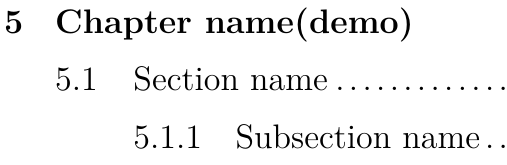
\includegraphics[width=0.5\linewidth]{tocStyleAlign_0_en.png}}
    
    \vspace{10mm}
    \subcaptionbox
        {中文樣板 \textbackslash{}def\textbackslash{}tocStyleAlign\{1\} }
        {
\includegraphics[width=0.35\linewidth]{tocStyleAlign_1_zh.png}}
    \hspace{10mm}
    \subcaptionbox
        {英文樣板 \textbackslash{}def\textbackslash{}tocStyleAlign\{1\} }
        {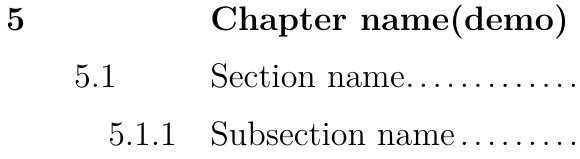
\includegraphics[width=0.5\linewidth]{tocStyleAlign_1_en.png}}
    \caption{樣板提供的目錄對齊風格}
    \label{fig:tocStyleAlign}
\end{figure}

\paragraph{目錄章級風格}
config.tex中的 tocStyleChapter 可以切換目錄章級的風格,如\cref{fig:tocStyleChapter}(中英文效果一樣,只貼中文),章級條目與上方拉開並使用粗體、不用點線。不過在僅有章級的區域(如摘要附近)若亦拉開則會顯得過疏。所以另提供介於中間的風格``1'',其效果如本教學,就不另外截圖了。
\begin{figure}
    \centering
    \subcaptionbox
        {\textbackslash{}def\textbackslash{}tocStyleChapter\{0\} }
        {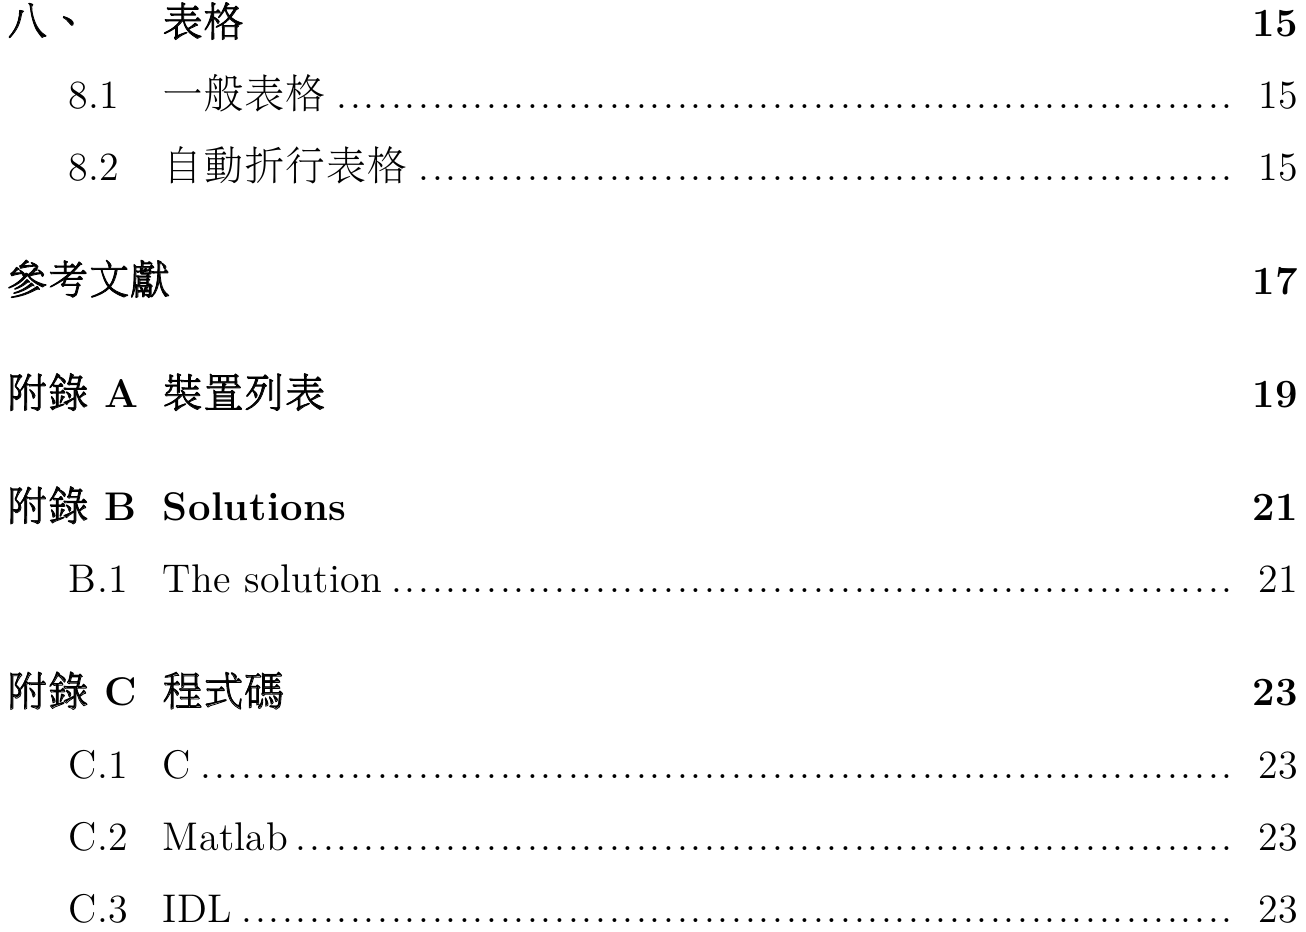
\includegraphics[width=0.6\linewidth]{tocStyleChapter_0.png}}
    
    \vspace{10mm}
    \subcaptionbox
        {\textbackslash{}def\textbackslash{}tocStyleChapter\{2\} }
        {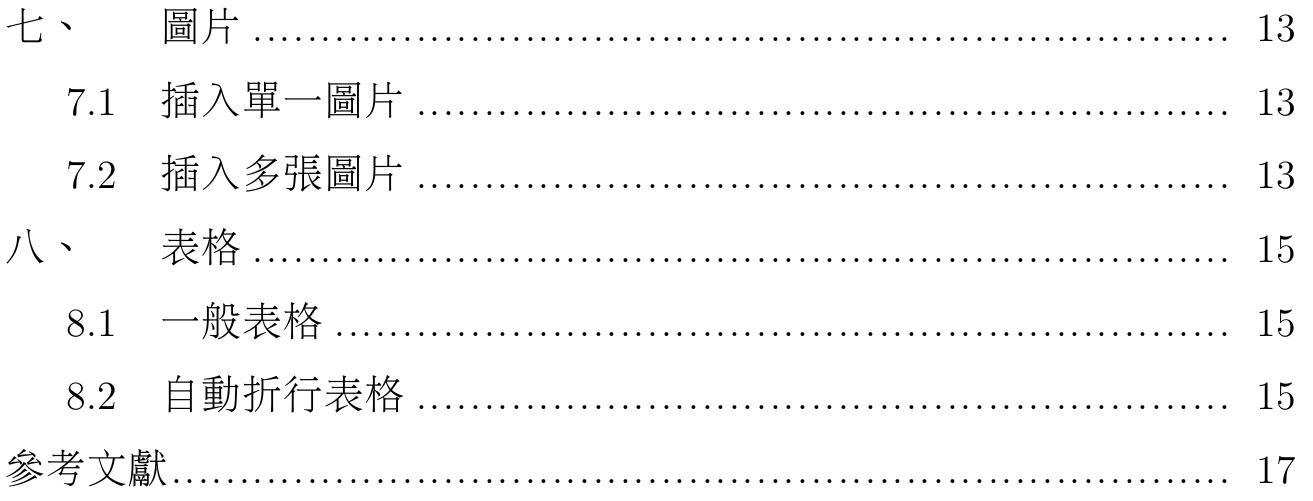
\includegraphics[width=0.6\linewidth]{tocStyleChapter_2.png}}
    \caption{樣板提供的目錄章級風格}
    \label{fig:tocStyleChapter}
\end{figure}

\subsubsection{標題風格}
標題風格提供三種形式讓各位自行選擇要採用哪一種。(下面的示範為避免影響到主文件章節數值,使用圖片展示編譯結果。)

首先示範使用\LaTeX\ 預設值(\textbackslash{}styletitles\{0\})的情況,如\cref{fig:titleStyle_0}:
\begin{figure}[!h]
    \centering
    \subcaptionbox
        {config.tex 中的設定}
        {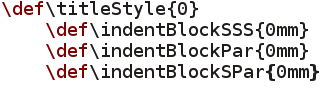
\includegraphics[width=0.3\linewidth]{titleStyle_c0.png}}
    
    \subcaptionbox
        {}
        {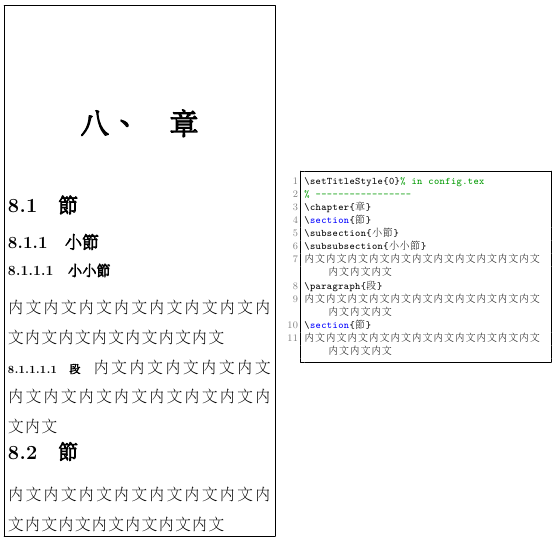
\includegraphics[width=0.8\linewidth]{titleStyle_0.png}}
    \caption{標題風格 \textbackslash{}def\textbackslash{}titleStyle\{0\}}
    \label{fig:titleStyle_0}
\end{figure}

接著是修改標題形式成學校樣式,但不進行縮排。如\cref{fig:titleStyle_1}
\begin{figure}[!h]
    \centering
    \subcaptionbox
        {config.tex 中的設定}
        {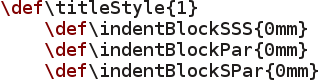
\includegraphics[width=0.3\linewidth]{titleStyle_c1.png}}
    
    \subcaptionbox
        {}
        {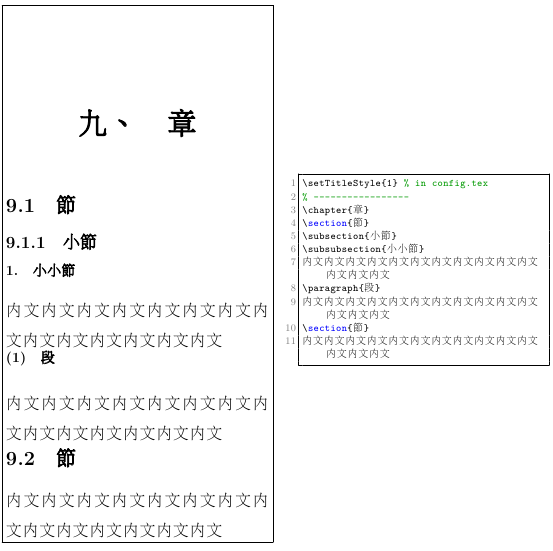
\includegraphics[width=0.8\linewidth]{titleStyle_1.png}}
    \caption{標題風格 \textbackslash{}def\textbackslash{}titleStyle\{1\}}
    \label{fig:titleStyle_1}
\end{figure}

最後是連縮排也符合學校規定(長度自訂)(\cref{fig:titleStyle_1i})。不過內文同時縮排須要調整\textbackslash{}leftskip的數值,目前樣板須要手動於縮排前後修改。並且記得以空行分隔上一個段落,否則無法產生效果。\textbackslash{}leftskip只有在碰到\textbackslash{}subsubsection層級之後才須要加,碰到的機會應該不多。
\begin{figure}[!h]
    \centering
    \subcaptionbox
        {config.tex 中的設定}
        {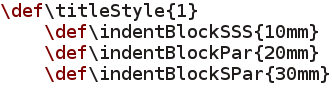
\includegraphics[width=0.3\linewidth]{titleStyle_c1i.png}}
    
    \subcaptionbox
        {}
        {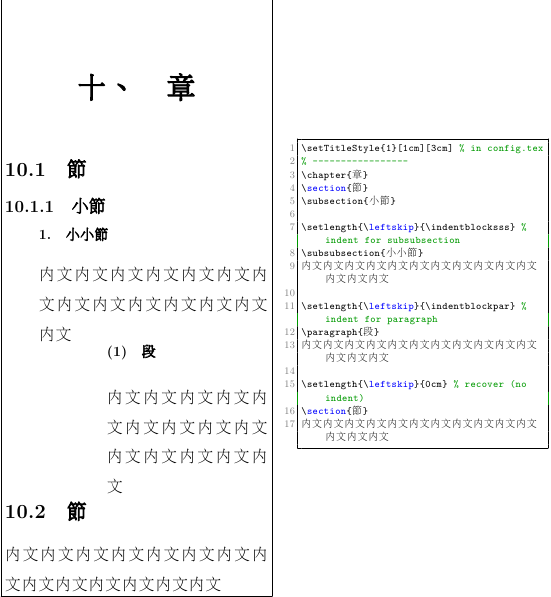
\includegraphics[width=0.8\linewidth]{titleStyle_1i.png}}
    \caption{標題風格 \textbackslash{}def\textbackslash{}titleStyle\{1\}與\textbackslash{}leftskip}
    \label{fig:titleStyle_1i}
\end{figure}

\chapter{樣板測試結果及已知問題}
照目前測試結果來看,TeX Live以及MiKTeX最新版(2016年)都能完美支援。
\label{sec:c_issue}
\section{測試結果}
\begin{table}[h]
    \centering
    \begin{tabularx}{\textwidth}{| X | X | l | X |}
        \hline
        Tex發行版 & 作業系統 & XeTeX 版本 & 測試結果 \\ \hline
        TeX Live 2012 \newline (2012.20120611-5) & Debian GNU/Linux  \newline wheezy(7.9) & 3.1415926-2.4-0.9998 & 章節標題後立即接圖片會導致整段粗體,插入任一行文字可解決。\textbackslash{}url跨頁會導致頁眉及中間浮動環境均含連結。listings 套件的行號距離會比設定值短。 \\ \hline
        TeX Live 2016 \newline(2016.20160819-2) & Debian GNU/Linux  \newline stretch/sid(9) & 3.14159265-2.6-0.99996 & 無問題 \\ \hline
        MiKTeX  \newline(???) & Window 7/8/10(en) & ??? & 無問題 \\ \hline
        TeX Live 2016   & Window 7 & ??? & 無問題 \\ \hline
    \end{tabularx}
\end{table}

\section{待解決問題}
%\todo[inline]{url package will load by biblatex. didn't work now.}
\begin{itemize}
 \item 過長的連結會超出頁邊。本樣板使用url 套件處理這個問題,但仍無法處理超長單字。目前breakurl套件(1.40+)提供了anythingbreaks選項,可以任意截斷連結,請參考\url{http://tex.stackexchange.com/questions/107507/biblatex-url-breaking-not-working-in-dvi-mode} 的說明。不過breakurl 僅支援原始的\LaTeX\ ,PDFLaTeX/XeLaTeX不支援。
\end{itemize}


\end{document}
